% chktex-file 44
\chapter[Identifying Transits in TrES Data Sets: The Human Factor]%
{%
Identifying Transits in \\ TrES Data Sets: \\ The Human Factor%
\protect\CFNF%
}\label{cha:human}

\section{Understanding the Yield of Transit Surveys}\label{cha:human:sec:intro}

The discovery of the first transiting planet \hdTZNb\ \citep{Charbonneau_Brown_Latham:apjl:2000a, Henry_Marcy_Butler:apj:2000a} spawned a great flurry of campaigns to search for these rare objects.
Transiting planets yield precise measurements of the radius and mass of giant planets outside our solar system that are much needed constraints for theoretical models, and they provide the promise of a better understanding of the structure and formation of gas giants.
\hdTZNb\ was first identified \citep{Mazeh_Naef_Torres:apj:2000a} as a Jupiter-mass planet by radial-velocity surveys of the solar neighborhood.
It was later observed to transit its star.
In comparison, the majority of transit surveys aimed to photometrically monitor $100,\!000$s of stars for evidence of transits.
Initial estimates \citep[see, e.g.,][]{Horne:ASP:2003a} of the yield of transiting planets from these surveys were optimistic during the initial rush of enthusiasm, with expectations of many new discoveries every month.
At the time of writing, seven years later, there are only 20 known transiting exoplanets.
Several transit surveys have overcome the difficulty in obtaining the photometric precision required to observe a 1\% transit over a large field of view for thousands of stars, and have proven their ability to identify transiting planets: the OGLE-III survey \citep{Udalski_Paczynski_Zebrun:acta:2002a}, the XO project \citep{McCullough_Stys_Valenti:pasp:2005a}, the HAT survey \citep{Bakos_Lazar_Papp:pasp:2002a}, the SuperWASP survey \citep{Street_Pollaco_Fitzsimmons:ASP:2003a}, and the Trans-atlantic Exoplanet Survey (TrES; \citealt{Alonso_Deeg_Brown:an:2004a, Dunham_Mandushev_Taylor:pasp:2004a, ODonovan_Charbonneau_Kotredes:AIP:2004a}).
Despite these successes, the anticipated flood of new transiting planets is still only a trickle.

Over time, we have developed a greater appreciation of additional factors that must be included in our predictions \citep[see][for a review]{Gaudi:asp:2007a}:
(i) Transit surveys are very biased toward large planets with short periods (Gaudi, Seager, \& Mallen-Ornelas~\citeyear{Gaudi_Seager_Mallen-Ornelas:apj:2005a}; \citealp{Gaudi:apjl:2005a}).
(ii) Many of the stars in a given field are giants or large dwarfs \citep{Brown:apjl:2003a}; hence transits of these large stars are not detectable by ground-based surveys with ten-centimeter telescopes.
(iii) The presence of systematics in the data, correlated on transit-like time scales, increases the signal-to-noise ratio requirement to detect a transit to beyond that derived from simple Poisson noise.
This increases the number of observed transits required to have a strong transit detection, and hence affects the choice of the length of the observing run for the field.

These factors affect the number of strong transit signals that are expected in the data.
However, when estimating the yield from a survey, we must account for how we detect these periodic signals.
There are two steps in my procedure for identifying candidate transiting systems.
First, I use an automated algorithm to find the statistically most significant transit signals.
Then, I view these strong signals and determine which are worth further analysis.
It is important that both steps are efficient in recovering transit signals.
Several algorithms have been proposed in the case of transit surveys \citep[see, e.g.,][for a review]{Tingley:aa:2003a, Tingley:aa:2003b}.
For the analysis of the TrES data, I use the Box-fitting Least-Squares (BLS) transit-search algorithm of \citeauthor*{Kovacs_Zucker_Mazeh:aa:2002a}~(\citeyear{Kovacs_Zucker_Mazeh:aa:2002a}, see appendix~\ref{cha:bls}), as do several other groups such as the HAT survey.
Several studies of the potential recovery rates of transit candidates have been done by transit surveys \citep[see, e.g.,][]{Gilliland_Brown_Guhathakurta:apjl:2000a, Bramich_Horne_Bond:mnras:2005a, Kane_Collier-Cameron_Horne:mnras:2005a, Weldrake_Sackett:apj:2005a}.
Here I present the recovery rate of the BLS algorithm when applied to TrES data.
I also discuss my ability to spot true transit signals among the noise, as the efficiency of this step has not been previously quantified.

\section[Injecting Model Light Curves into a TrES Data Set]{Injecting Model Light Curves into a \\ TrES Data Set}\label{cha:human:sec:model}

I conducted a blind test of my ability to identify transit-like signals in a real data set from the TrES campaign.
I chose the TrES Lyr1 field (centered on the star \mbox{16\,Lyr}) in which I had identified the transiting planet \tresTwo\ (\citealp{ODonovan_Charbonneau_Mandushev:apjl:2006a}, see chapter~\ref{cha:tres2}).
The total yield to date of this $5.7\degr \times 5.7\degr$ field, which contains 27,446 stars, is one confirmed planet.

\begin{figure}
\begin{center}
\centering
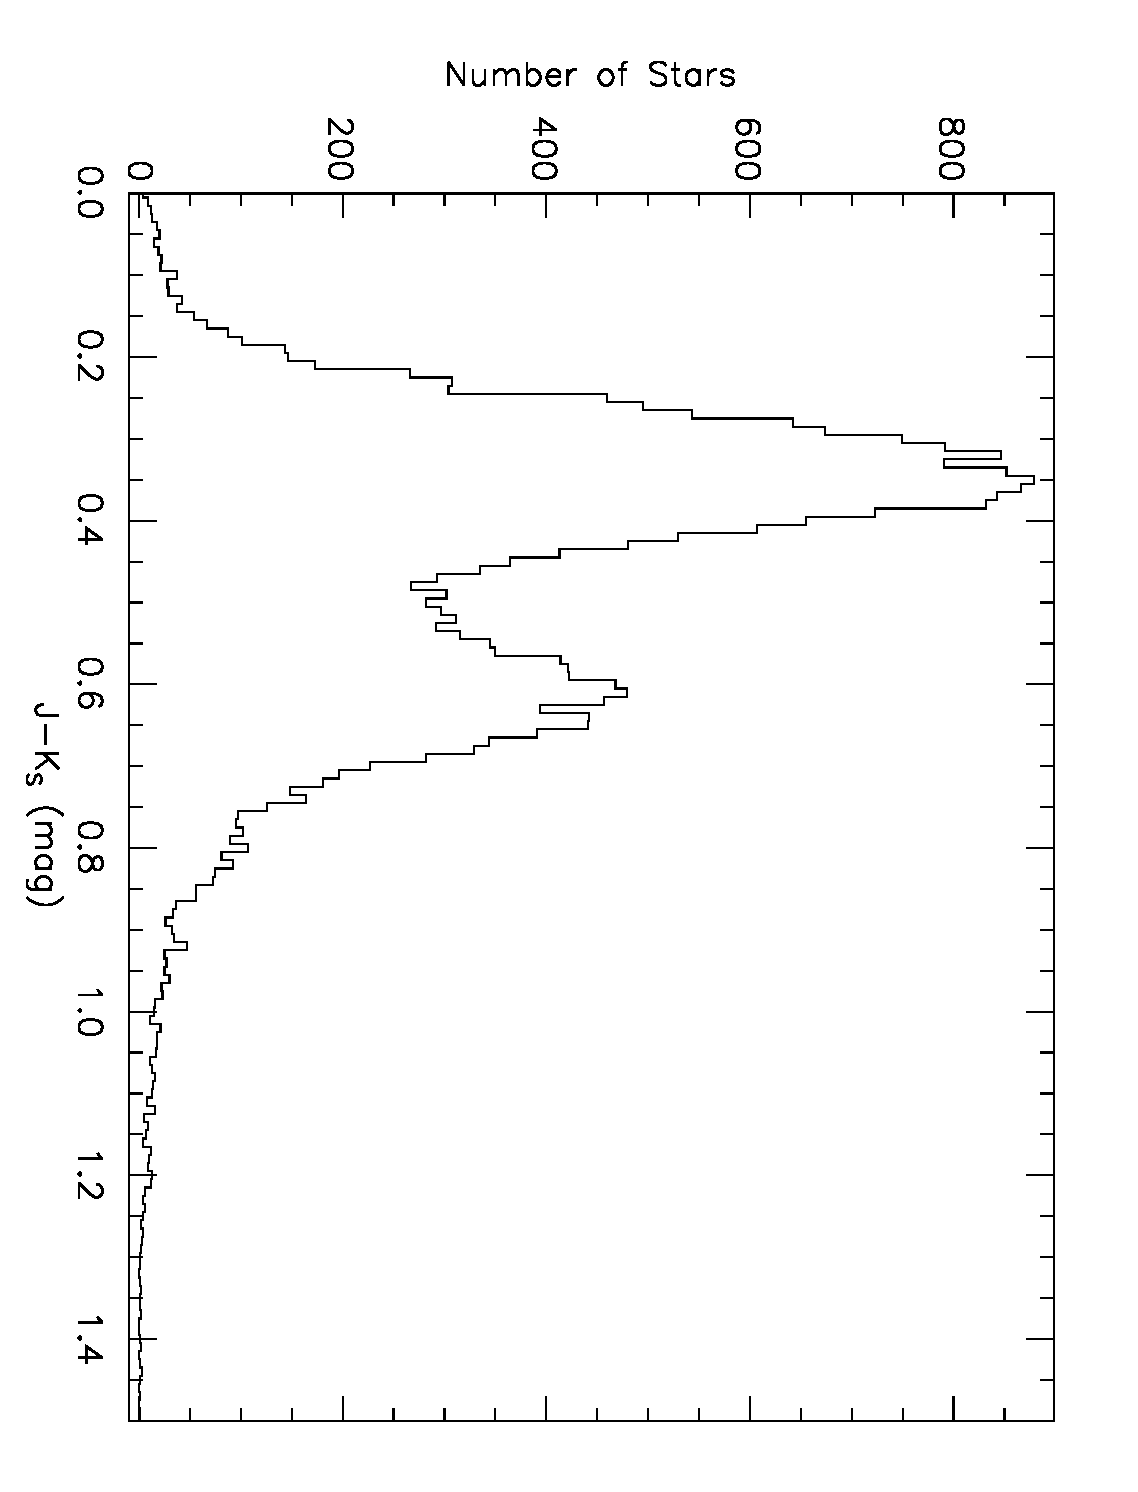
\includegraphics[width=.75\textwidth, angle=90]{7_jmks}\\
\caption[Histogram of 2MASS $J-K_{s}$ for TrES Lyr1 field]{%
Histogram of the 2MASS $J-K_{s}$ infrared colors for the TrES Lyr1 field.%
}\label{cha:human:sec:model:fig:jmks}
\end{center}
\end{figure}

\begin{figure}
\begin{center}
\centering
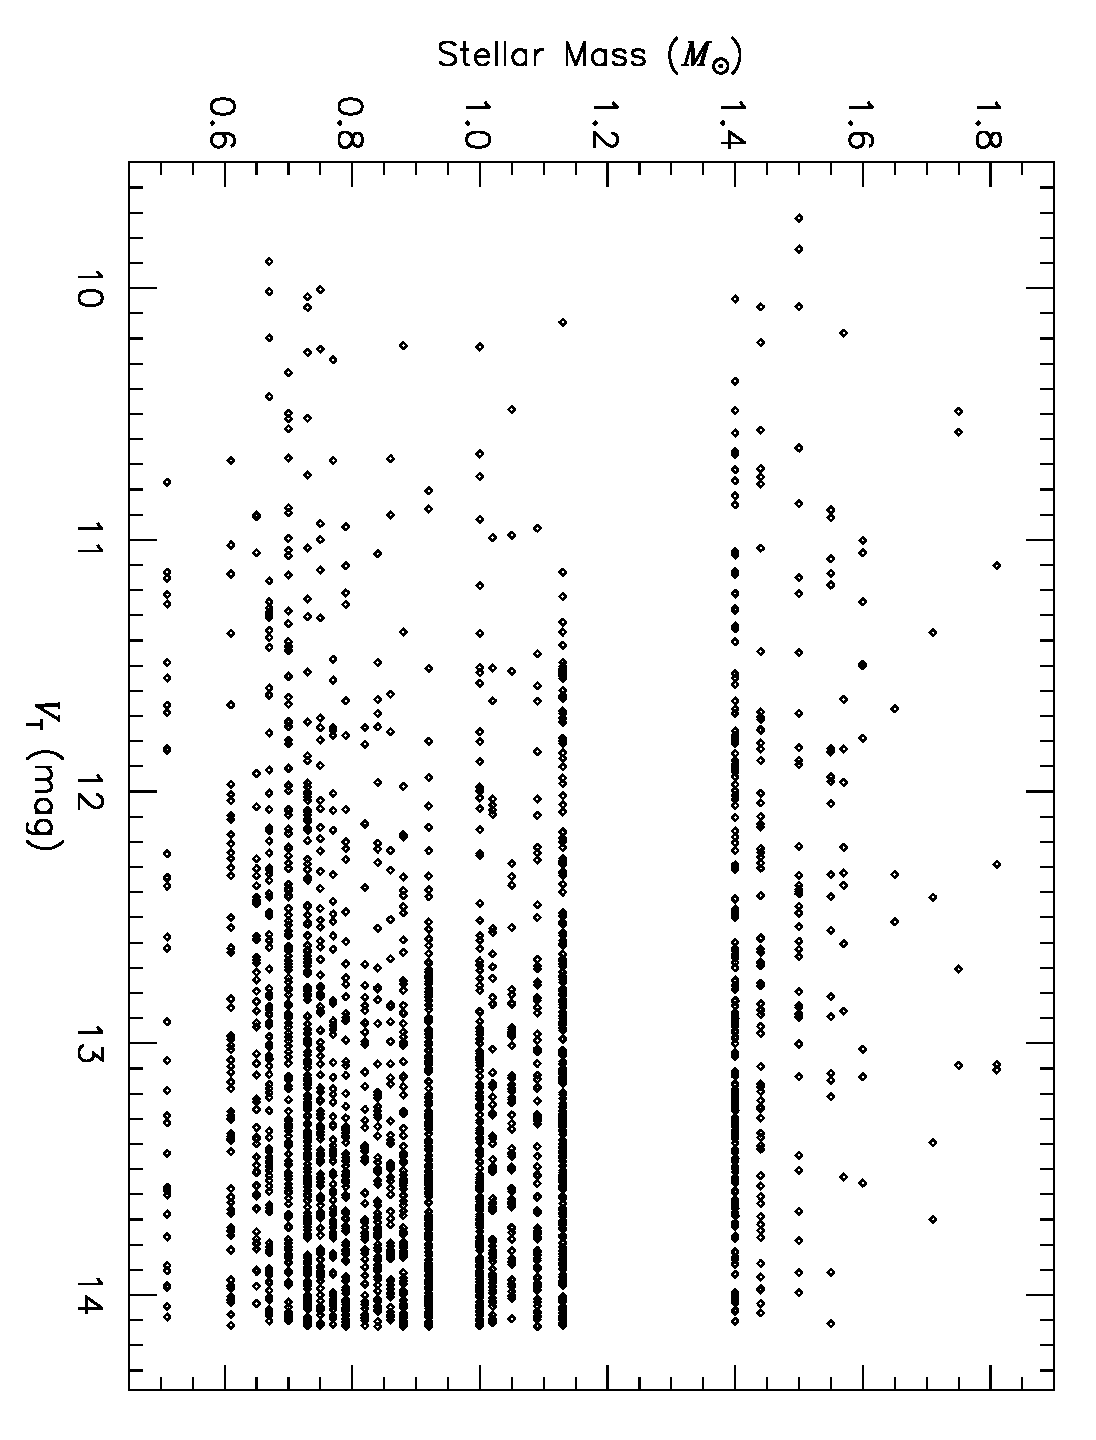
\includegraphics[width=.60\textwidth, angle=90]{7_phys_a}\\
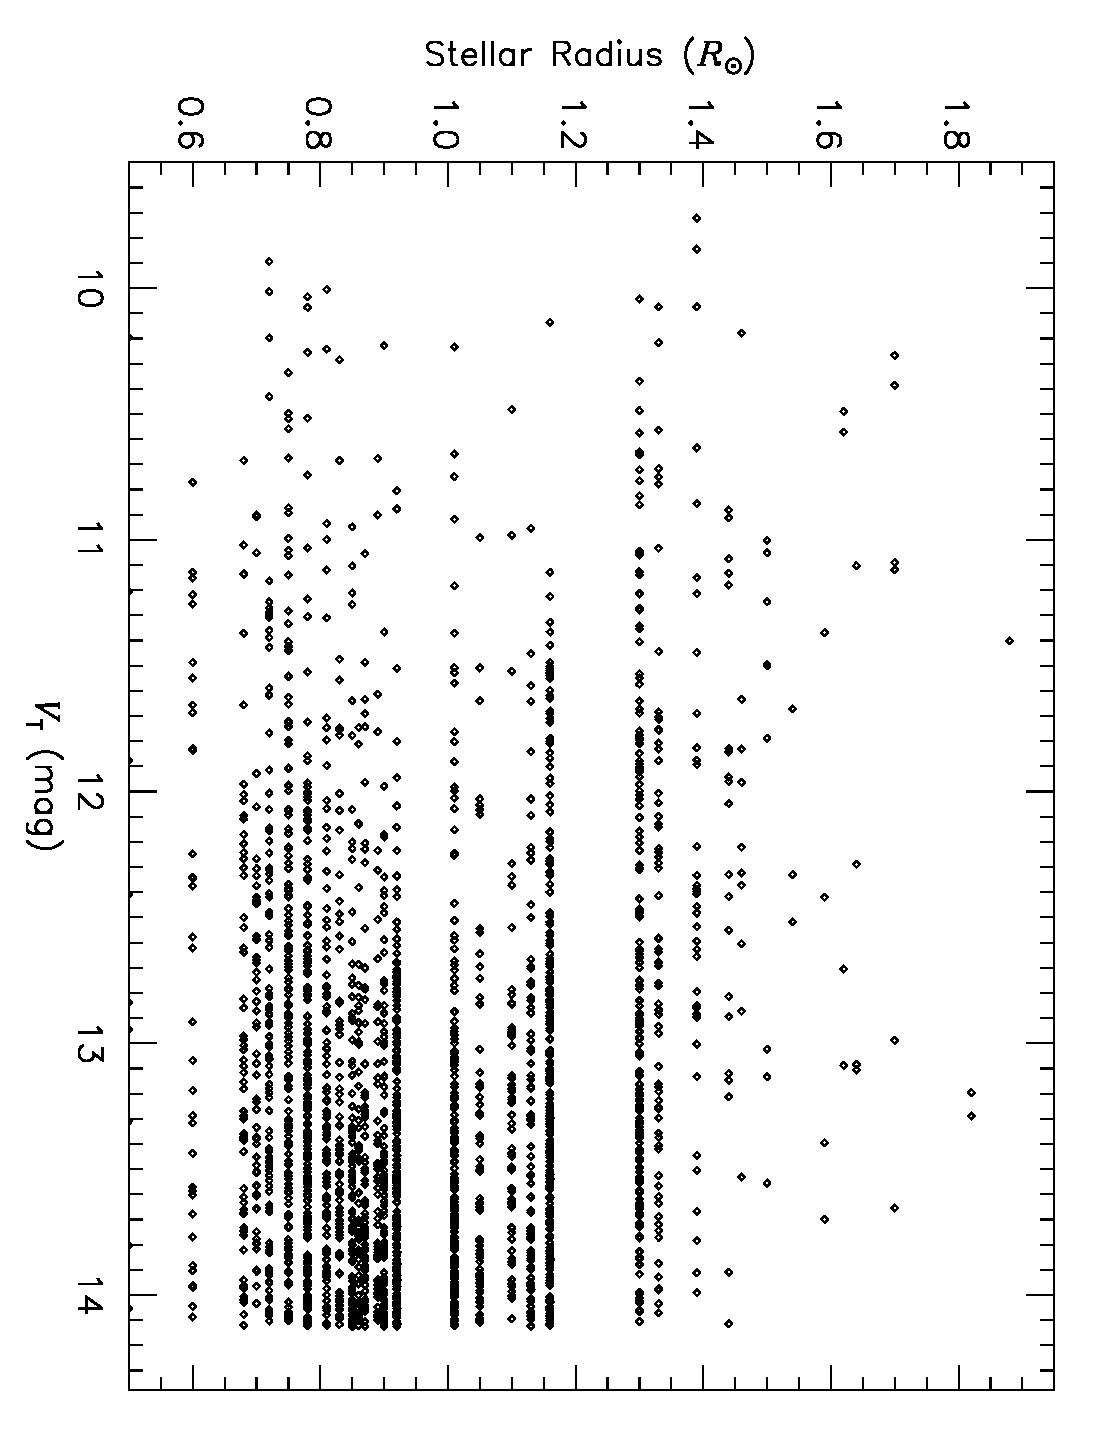
\includegraphics[width=.60\textwidth, angle=90]{7_phys_b}\\
\caption[Randomized stellar parameters for injected transits]{%
Randomized stellar parameters used to generate fake transit light curves injected into a TrES time series, plotted versus the approximate $V_{T}$ magnitudes: %
({\textit top panel}) the mass of the host star, and %
({\textit bottom panel}) the stellar radius.
The number of stars of a given magnitude increases with magnitude.
The stellar mass and radius were generated using the 2MASS $J-K_{s}$ infrared colors from figure~\ref{cha:human:sec:model:fig:jmks} (see text for a discussion of the distribution).
These values were computed to two decimal places, which results in the discrete levels visible in the plots.%
}\label{cha:human:sec:model:fig:stel}
\end{center}
\end{figure}

\begin{figure}
\begin{center}
\centering
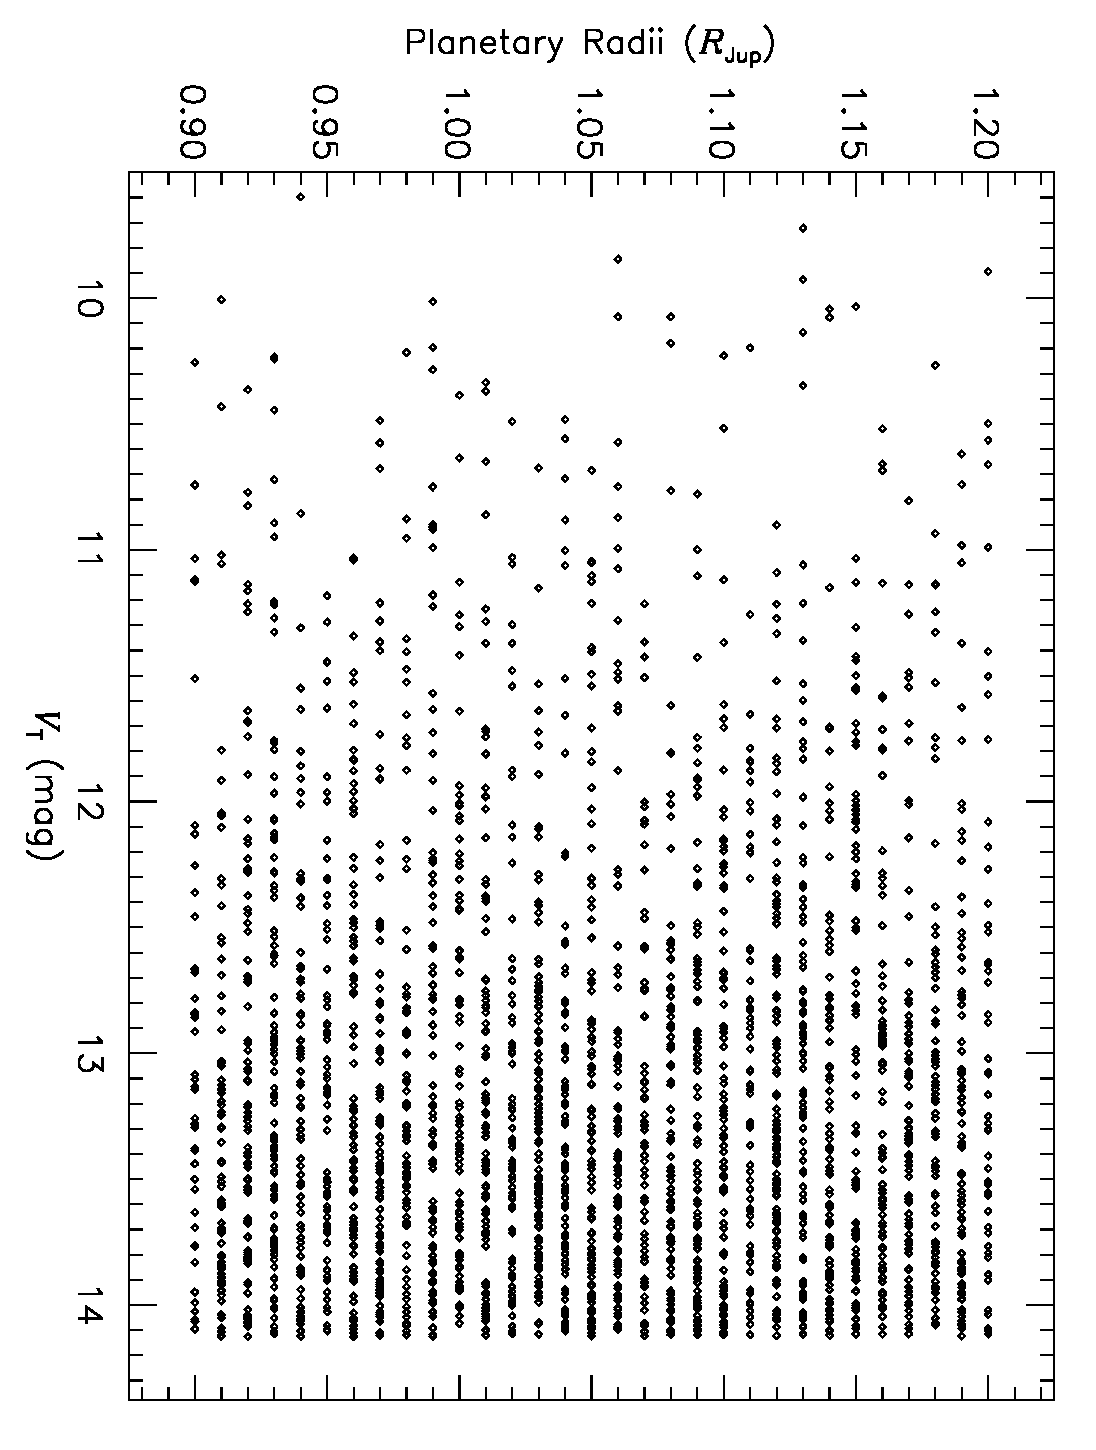
\includegraphics[width=.75\textwidth, angle=90]{7_phys_c}\\
\caption[Randomized planetary parameters for injected transits]{%
Same as for figure~\ref{cha:human:sec:model:fig:stel}, but for the radius $R_{p}$ of the supposed transiting planet.
Again, the discrete levels in the values for $R_{p}$ are due to the limit of two decimal places for the values.
%
}\label{cha:human:sec:model:fig:plan}
\end{center}
\end{figure}

First I generated a list of parameters for fake transit light curves as follows.
Note that I did not consult this parameter list until I had attempted to visually identify all of the fake candidate transiting planets.
As part of the standard TrES analysis pipeline (\citealp[see, e.g.,][]{Dunham_Mandushev_Taylor:pasp:2004a}; \citealp{ODonovan_Charbonneau_Torres:apj:2006a}, see chapter~\ref{cha:gsc}; \citealp{ODonovan_Charbonneau_Alonso:apj:2007a}, see chapter~\ref{cha:and0}).
I had previously generated a list of 27,446 stars present in the Lyr1 field, ordered by instrumental $r$ magnitude.
The position of a star in this list, starting at 0 for the brightest star, is the ``star number'' for this star.
In order to span a wide range of transit parameters, I would need to inject a large number of fake transits.
However, I would also need to somewhat simulate the scarcity of real transit signals in the data.
I decided to choose a random%
\footnote{%
The random numbers discussed in this chapter were generated using IDL's \textit{RANDOMU} function that generates uniformly distributed, pseudo-random numbers using the method of~\citet{Park_Miller:ACM:1988a}.%
}%
\ number of fake transits to be injected, such that this number was $\sim$10\% of the total number of stars.
I then chose this number (2,612) of stars at random from the star list to be the ostensible candidate hosts of transiting planets.
From the 2MASS \citep{Cutri_Skrutskie_van-Dyk:2003a} $J-K_{s}$ infrared colors of these stars (see figure~\ref{cha:human:sec:model:fig:jmks}), I derived the stellar masses $M_{\star}$ and radii $R_{\star}$, assuming these to be dwarf stars and using an interpolation%
\footnote{%
The gaps in the stellar masses and radii were caused by a bug in the interpolation code that was not discovered until the hidden parameter file was examined after the analysis.
Future analysis will correct this.
However, I decided that the stellar radii (the more interesting parameter) cover a wide enough parameter space for my initial analysis.%
}%
\ of values from \citet{Cox::2000a}.
Note that since most of the stars with large $J-K_{s}$ values are in fact giants, the assumption that these stars are main-sequence stars (with small stellar radii corresponding to their color) leads to a bias toward identifying transiting planets that are too small to be detected if transiting giant stars.
The scarcity of radii $\rstar<0.65\,\rsun$ and $\rstar>1.40\,\rsun$ (and the similar dearth in masses) is the result of the 2MASS color distribution of figure~\ref{cha:human:sec:model:fig:jmks}.
I produced a random distribution of radii $R_{p}$ for the supposed planetary companions of these stars, where $0.9\leq R_{p} \leq 1.2\,R_{\mathrm Jup}$ based on the distribution of radii for the known transiting planets (see figure~\ref{cha:intro:sec:methods:sub:trans:fig:tp}).
The values for these three physical parameters are shown in figures~\ref{cha:human:sec:model:fig:stel} and~\ref{cha:human:sec:model:fig:plan}.

\begin{figure}
\begin{center}
\centering
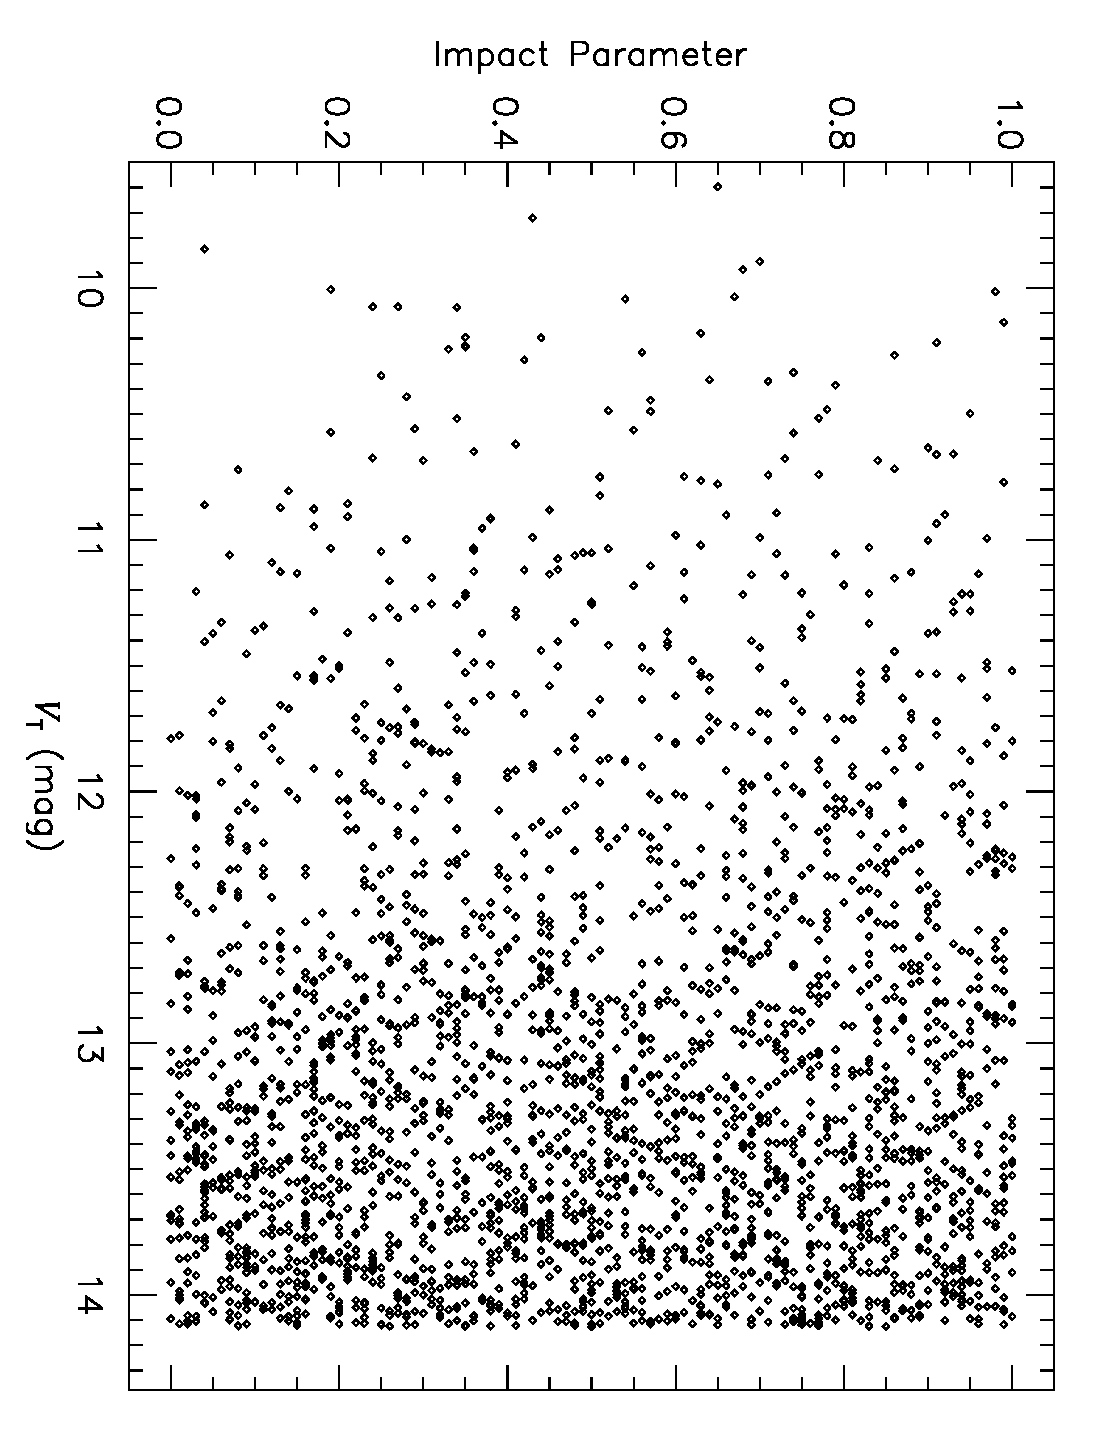
\includegraphics[width=.55\textwidth, angle=90]{7_orb_a}\\
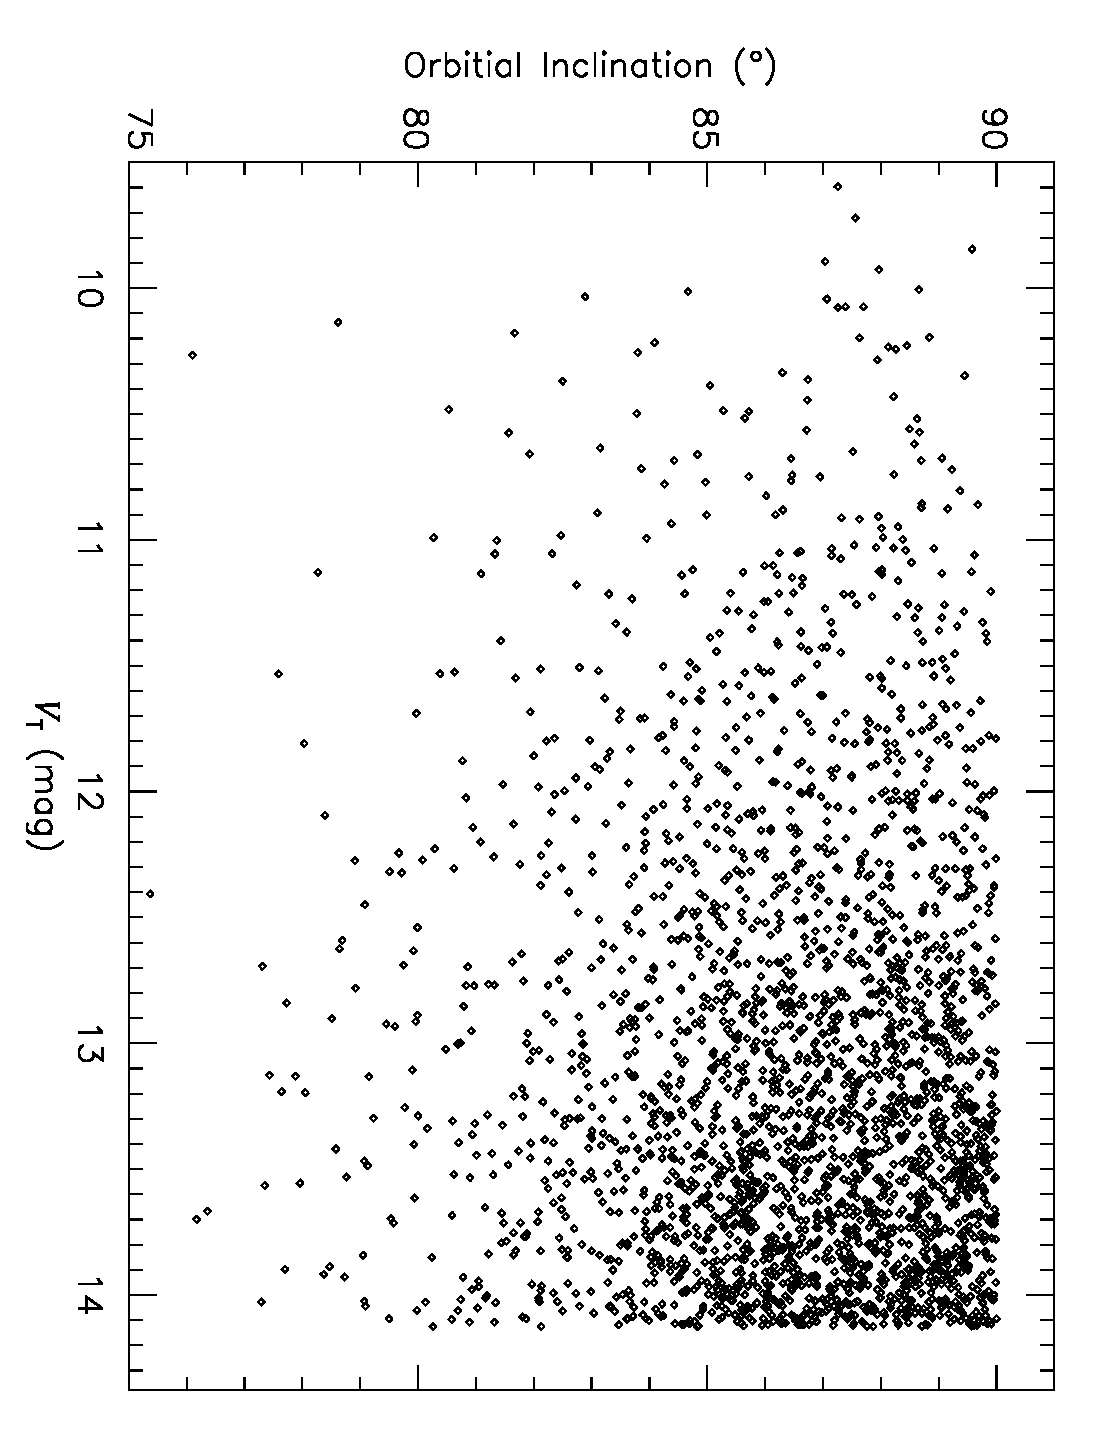
\includegraphics[width=.55\textwidth, angle=90]{7_orb_b}\\
\caption[Randomized transit impact parameters and orbital inclinations]{%
Randomized impact parameters ({\textit top panel}) for the model
transiting systems, from which the orbital inclinations in the {\textit bottom panel} are derived.
The orbital inclination is only significantly lower than $90\degr$ for those candidates with short periods and large impact parameters.
For example, if $i<80\degr$, $P=1$\,day, and $R_{\star}=R_{\sun}$, then $b$ must be greater than 0.7. %
}\label{cha:human:sec:model:fig:orb}
\end{center}
\end{figure}

I then computed random values for the transit impact parameter $b$ ($0\leq b\leq 1$).
From $b$, we can derive the orbital inclination $i= \arccos{(b R_{\star}/a)}$, where $a$ is the orbital semi-major axis computed using Newton's revised version of Kepler's third law.
The distribution of $b$ and $i$ can be seen in figure~\ref{cha:human:sec:model:fig:orb}.

\begin{figure}
\begin{center}
\centering
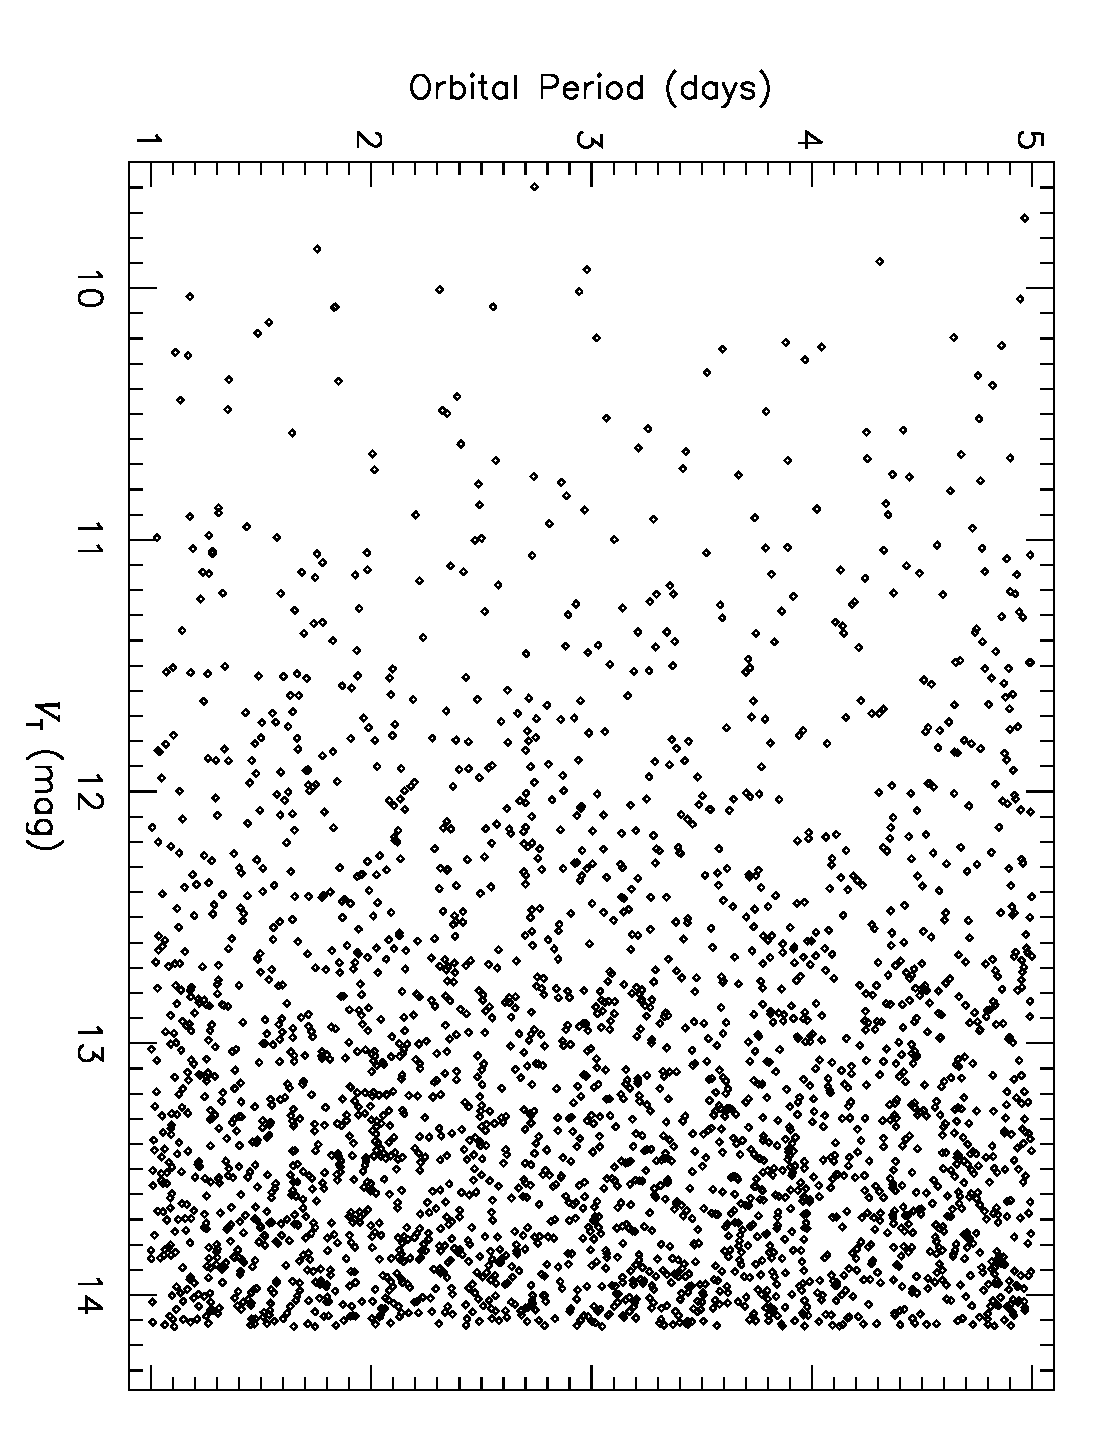
\includegraphics[width=.55\textwidth, angle=90]{7_bls_a}\\
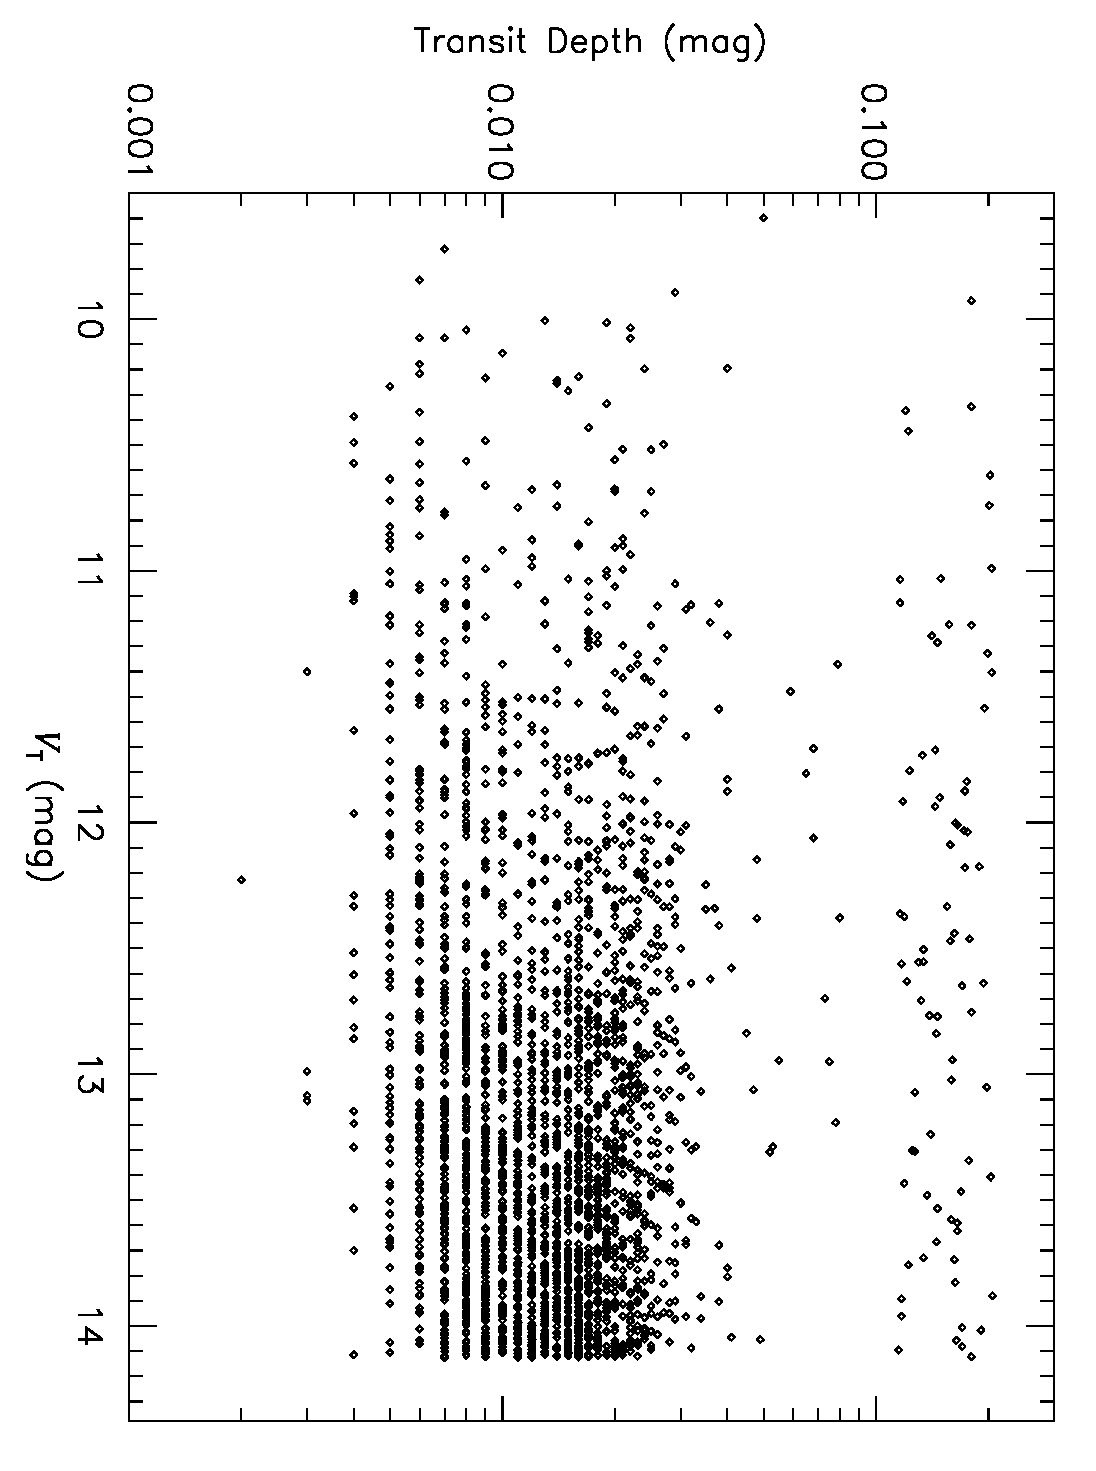
\includegraphics[width=.55\textwidth, angle=90]{7_bls_b}\\
\caption[Randomized values for first two BLS parameters]{%
Randomized values for two of the four parameters that are derived for each light curve by the Box-fitting Least-Squares (BLS) transit-search algorithm: %
({\textit top panel}) the orbital period $P$ of the transit, and %
({\textit bottom panel}) the transit depth $\Delta$.
To mimic the output of the BLS algorithm, $P$ and $\Delta$ are kept to 6 and 3 decimal places, respectively.
Since \mbox{$0.9\,\rjup \leq \rp \leq 1.2\,\rjup$} and most derived stellar radii lie in the range \mbox{$0.7\,\rsun \leq \rstar \leq 1.3\,\rsun$}, most of the transit depths are in the range \mbox{$0.005 \leq \Delta \leq 0.03$}.
The outliers are those transits of a very small star by very large planet, or of a very large star by a very small planet.
These points are evidence of the aforementioned bias caused by the assumption that all field stars are dwarf stars. %
}\label{cha:human:sec:model:fig:bls1}
\end{center}
\end{figure}

\begin{figure}
\begin{center}
\centering
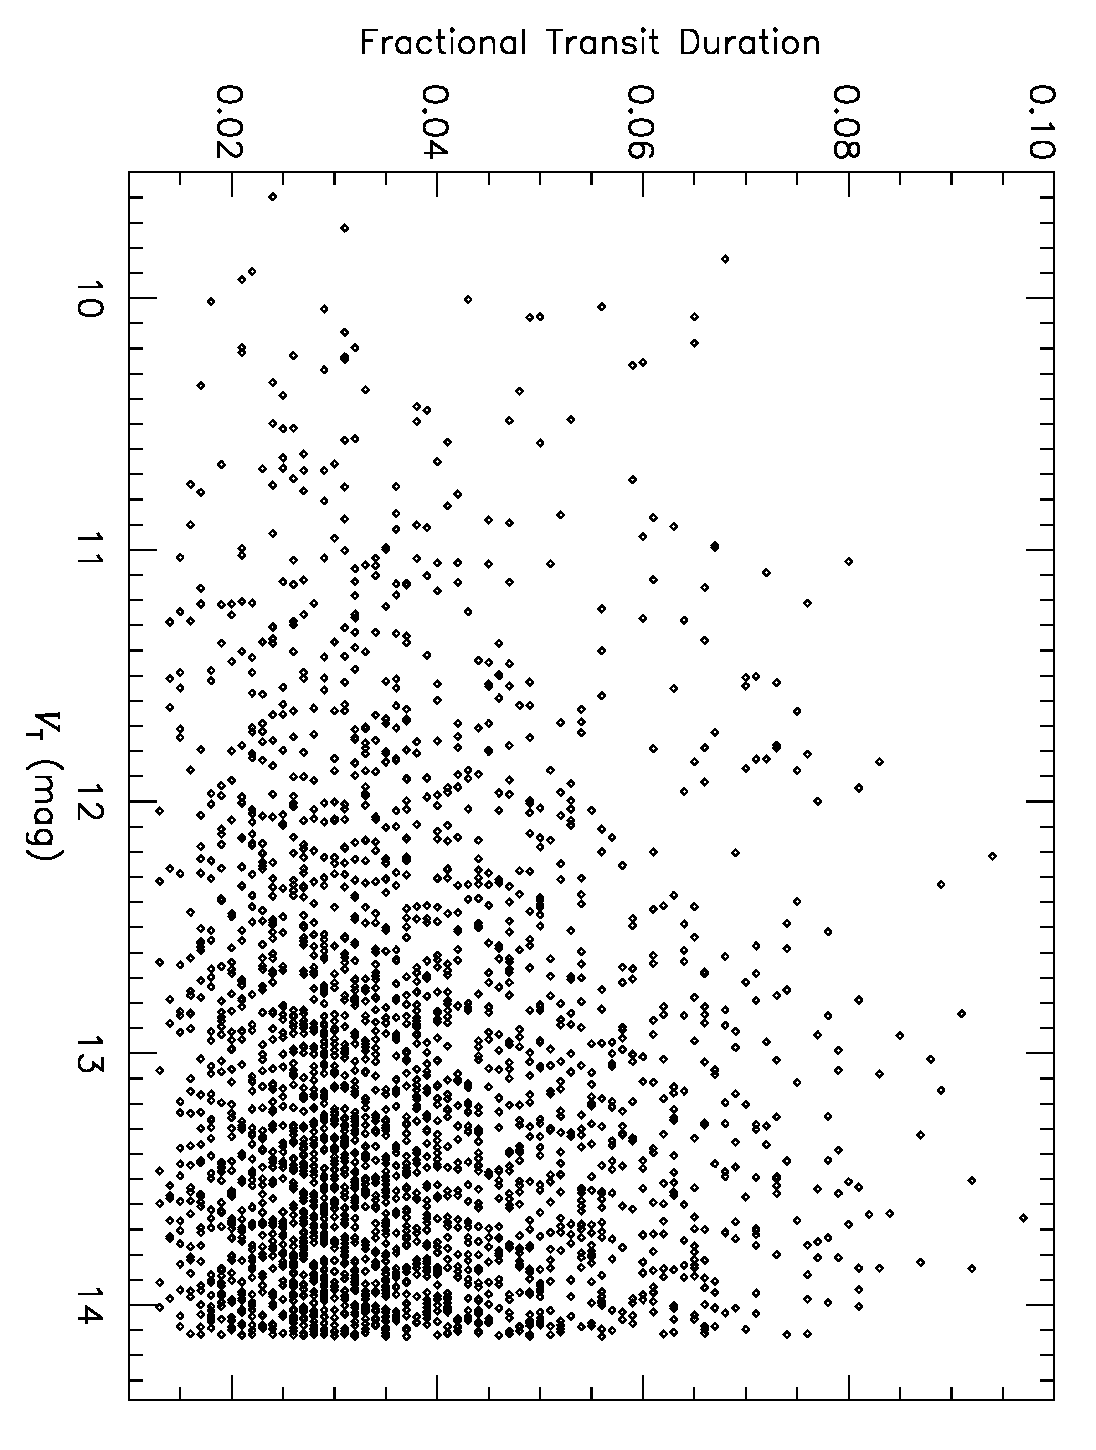
\includegraphics[width=.55\textwidth, angle=90]{7_bls_c}\\
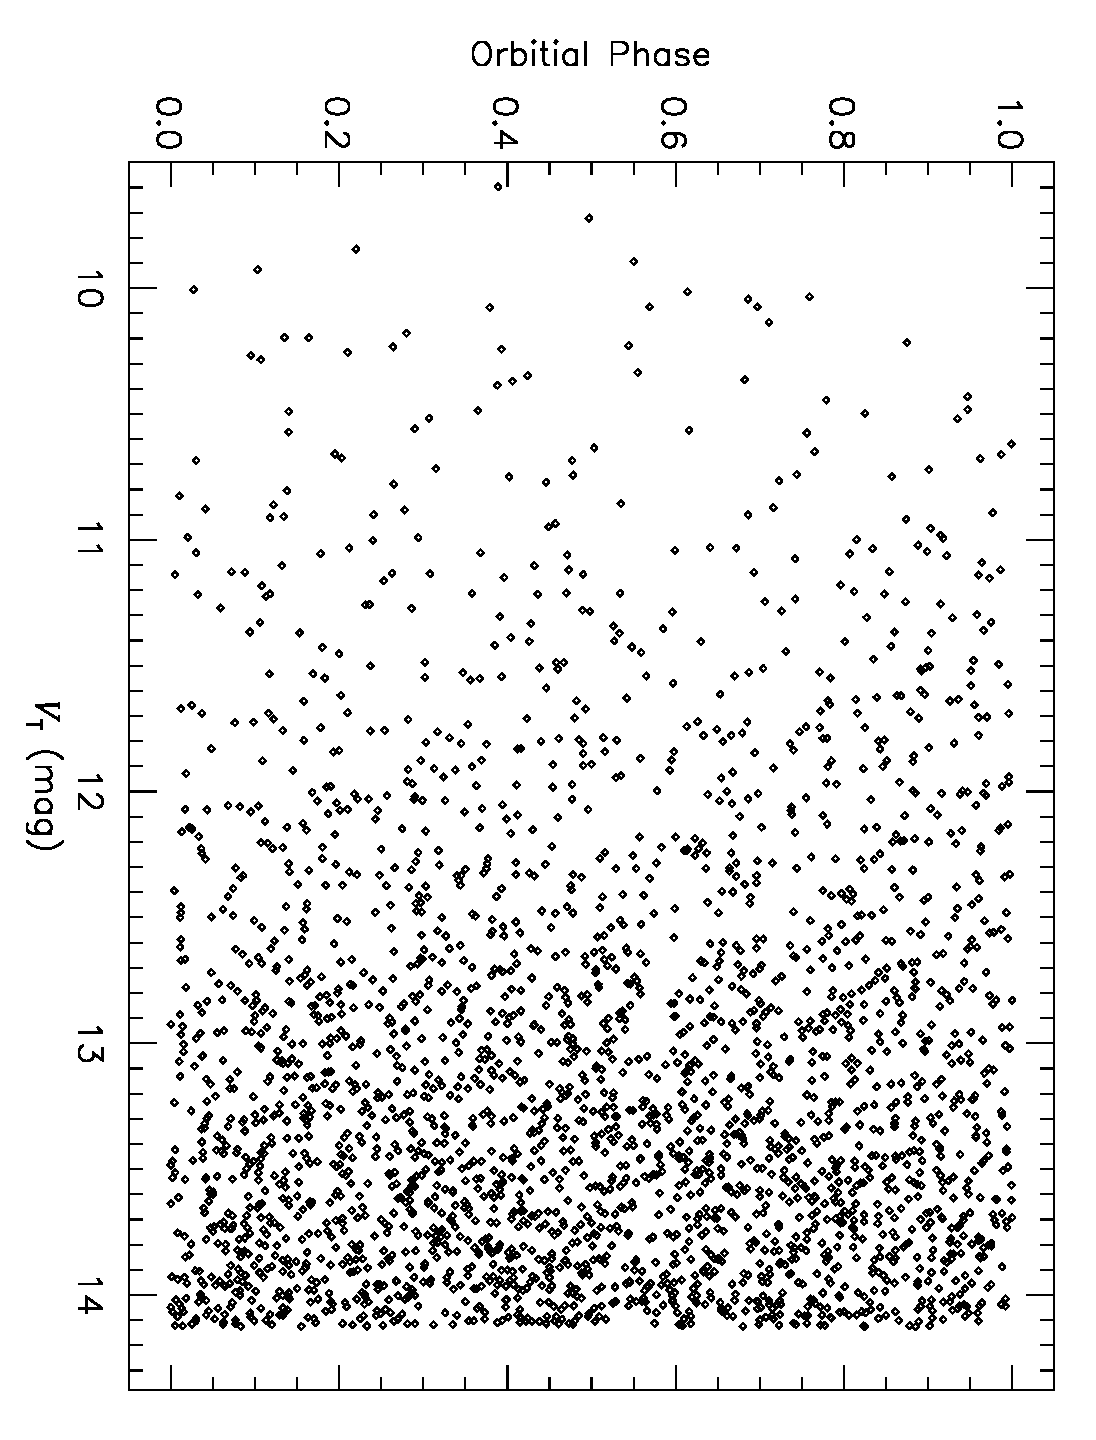
\includegraphics[width=.55\textwidth, angle=90]{7_bls_d}\\
\caption[Randomized values for final two BLS parameters]{%
Same as for figure~\ref{cha:human:sec:model:fig:bls1}, but for %
({\textit top panel}) the fractional transit duration $d$, and %
({\textit bottom panel})  the orbital phase $\Phi$ at the time of transit.
To mimic the output of the BLS algorithm, $d$ and $\Phi$ are kept to 3 decimal places.
The fractional transit duration is only significantly higher than $0.06$ for those candidates with short periods and small stellar radii.
For example, if $d=0.1$, then $a$ must be approximately $3\,R_{\star}$. %
%
}\label{cha:human:sec:model:fig:bls2}
\end{center}
\end{figure}

The BLS transit-search algorithm computes four transit parameters for every input light curve: the orbital period $P$ of the transit, the depth $\Delta$, the fractional duration $d = D/P$ (where $D$ is the duration), and the orbital phase $\Phi$ at the time $T_{c}$ of the transit center.
I generated random values for $P$ ($1\leq P \leq5$\,days; again see figure~\ref{cha:intro:sec:methods:sub:trans:fig:tp}) %
and $\Phi$ ($0\leq \Phi \leq 1$).
Note that while $\Phi$ is normally defined so that $\Phi=0$ at $T_{c}$, here $\Phi$ is defined so that $\Phi=0$ at the start of the TrES observing run.
This is to conform with the definition used by our BLS algorithm for $T_{c}$.
I derived the transit depths from $\Delta = (R_{p}/R_{star})^{2}$, and the fractional transit durations using equation~4 from \citet{Charbonneau_Winn_Latham:apj:2006a}:
\begin{eqnarray*} \label{cha:human:sec:model:eqn:dur}
\sin{i} \cos{\left(\frac{\pi D}{P}\right)} & = & \sqrt{1 - \left(\frac{R_{\star}+R_{p}}{a}\right)^{2}}, \\
 i\sim90\degr \Rightarrow d & = & \frac{1}{\pi} \arccos{\left(\sqrt{1 - \left(\frac{R_{\star}+R_{p}}{a}\right)^{2}}\right)}.
\end{eqnarray*}
Figures~\ref{cha:human:sec:model:fig:bls1} and~\ref{cha:human:sec:model:fig:bls2} shows the distribution of the parameters that should be recovered by the BLS algorithm.
\begin{figure}
\begin{center}
\centering
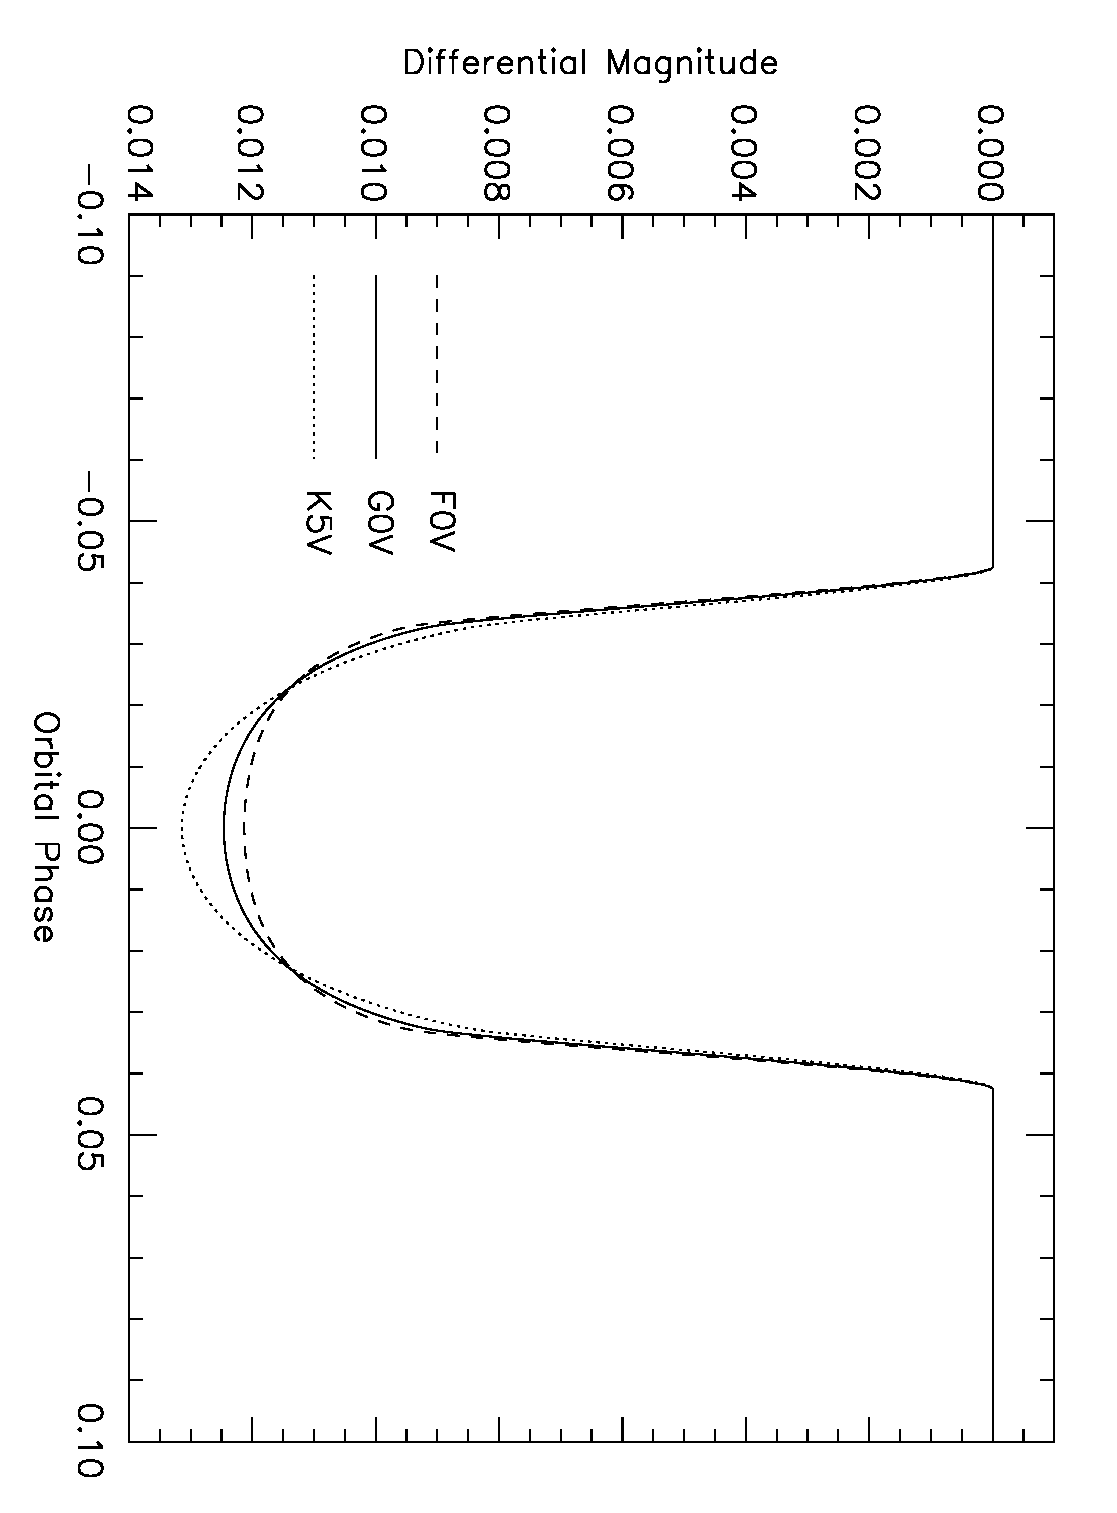
\includegraphics[width=.55\textwidth, angle=90]{7_agol_a}\\
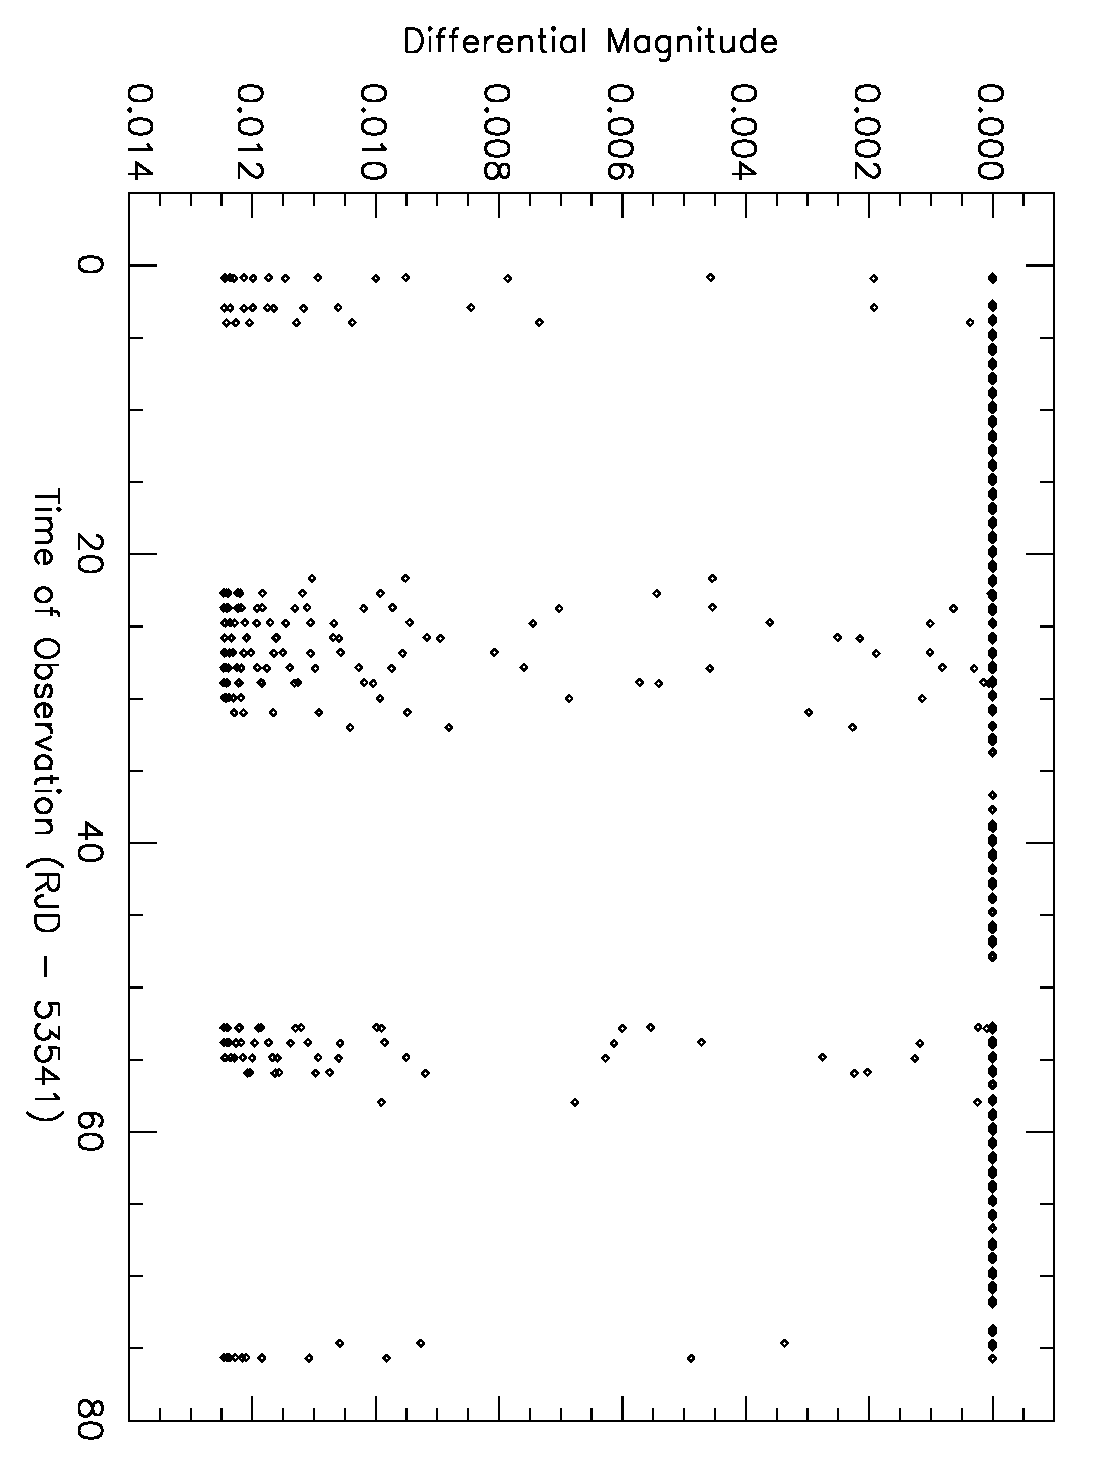
\includegraphics[width=.55\textwidth, angle=90]{7_agol_b}\\
\caption[Example of model transits]{%
({\textit Top}) %
Model transit light curves for a 1.2\% transit with a period of 1.038588\,days.
The shape of the three light curves is determined by the limb-darkening associated with the specified spectral type.
Distinguishing between these light curves is not possible for the TrES photometry, hence I simply assumed the G0V limb-darkening coefficients.
({\textit Bottom}) Model transit light curve from the {\textit top panel} plotted versus the times of observation during the TrES Lyr-1 run. %
}\label{cha:human:sec:model:fig:agol}%
\end{center}
\end{figure}

\begin{figure}
\begin{center}
\centering
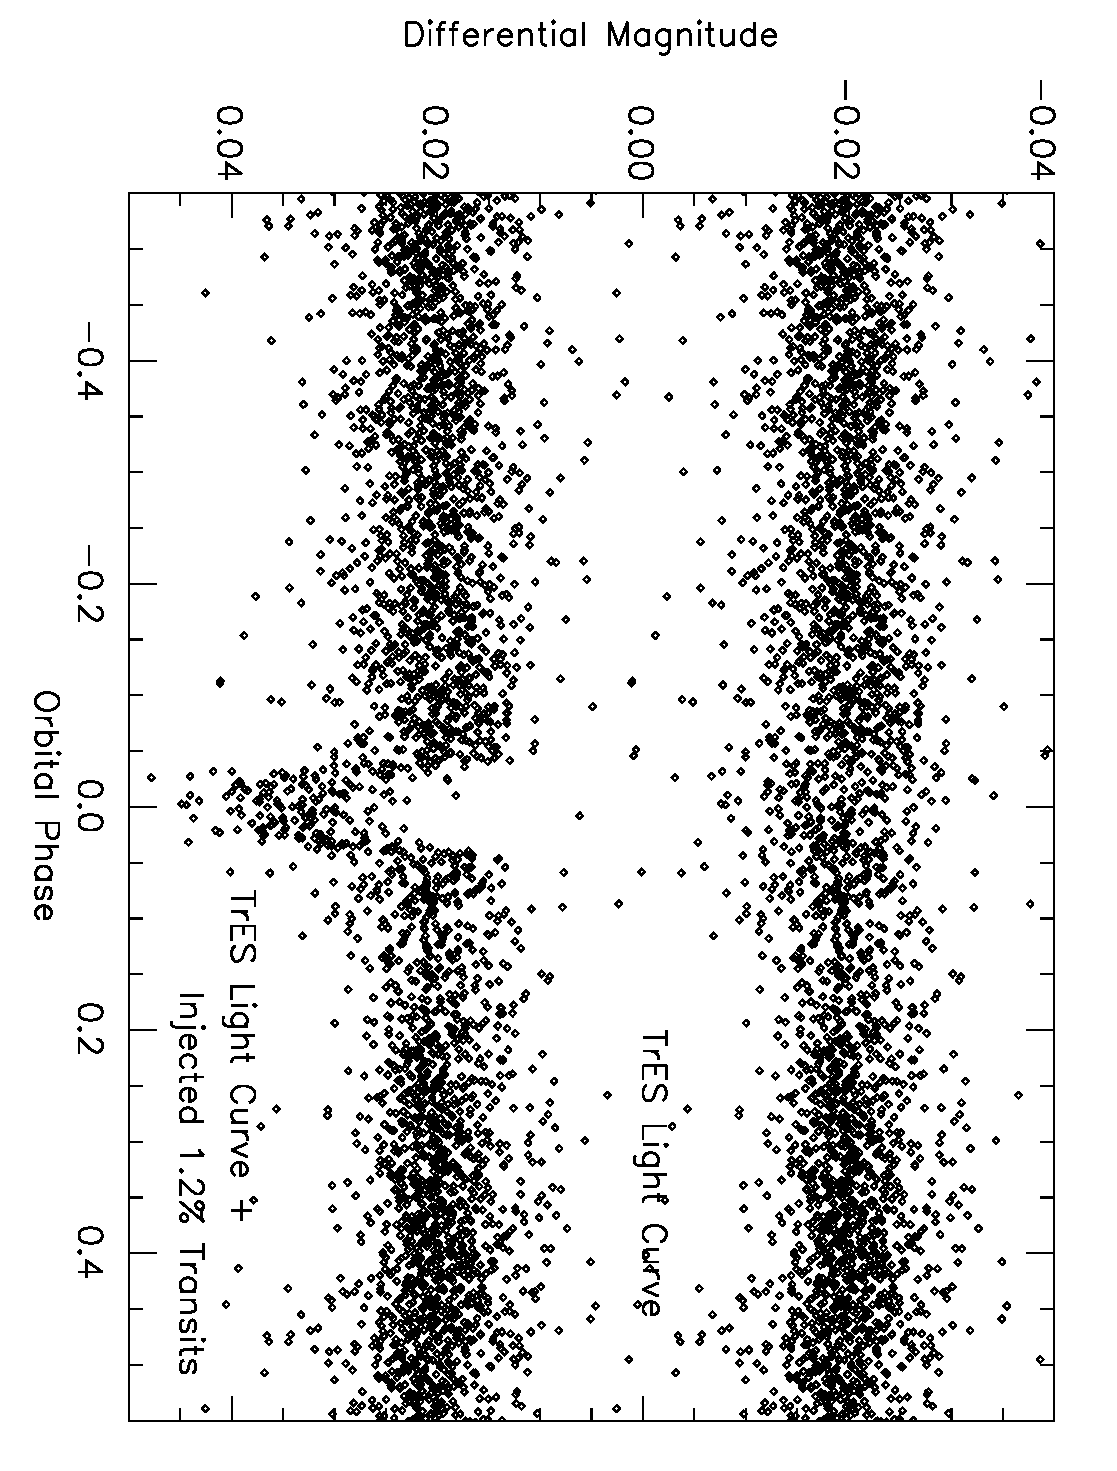
\includegraphics[width=.75\textwidth, angle=90]{7_agol_c}\\
\caption[Example of TrES light curve with injected transits]{%
The {\textit top} light curve is from the TrES Lyr1 field, phased to an orbital period of 1.038588\,days. The {\textit bottom} light curve shows the results of injecting the model transits from figure~\ref{cha:human:sec:model:fig:agol}%
.%
}\label{cha:human:sec:model:fig:inject}%
\end{center}
\end{figure}

Using these random system parameters as unseen input, I generated model transit light curves using code based on the analytic formulae of \citet{Mandel_Agol:apjl:2002a}.
This code computes the variation with time in the amount of obscuration of a limb-darkened source by a dark body, by deriving the area of the source obscured at that time, and outputs this variation in terms of relative flux.
Although the TrES photometry is too noisy to discern between different limb-darkening due to different stellar spectral types, the code requires limb-darkening coefficients as part of the input.
I assumed a quadratic limb-darkening model of the form:
\begin{eqnarray*}\label{cha:human:sec:model:eqn:limb}
I(\mu)/I(1) = 1-a(1-\mu)-b(1-\mu)^2,
\end{eqnarray*}
where $\mu=\cos{\gamma}$, $\gamma$ is the angle between the line of sight and the local normal to the stellar surface, $I$ is the specific intensity, and $a$ and $b$ are the limb-darkening coefficients.
The $R$-band quadratic limb-darkening coefficients for a G0V star (a typical spectral type from my data; see figure~\ref{cha:human:sec:model:fig:jmks}) are $a=0.2938$ and $b=0.3441$ ($T_{\mathrm eff}=6000$\,K, $\log{g}=4$, [Fe/H]=0, $V_{\mathrm turb}=0\,\kms$; \citealt{Claret:aa:2000a}).
figure~\ref{cha:human:sec:model:fig:agol} %
shows a phased model light curve using these coefficients and assuming $R_{p}/R_{\star}=0.1$.
figure~\ref{cha:human:sec:model:fig:agol} %
also shows model light curves displaying limb-darkening associated with a K5V and F0V star.
Distinguishing between the different limb-darkening requires photometry with exquisite precision (such as seen in \citealt{Brown_Charbonneau_Gilliland:apj:2001a}).
I simply assumed a G0V spectral type and luminosity class for my analysis.

I then accounted for the actual temporal coverage of the observations.
The effect of this can be seen in the {\textit bottom panel} of figure~\ref{cha:human:sec:model:fig:agol}%
, where the model from the {\textit top panel} have been plotted versus the times of observation of the Lyr1 field.
The final product of the TrES pipeline is a series of light curves, one for each star in the field.
These light curves have been decorrelated to remove systematics suffered by wide-field transit surveys, and averaged (in 9-minute bins) to reduce the computational effort of the BLS transit search.
For this test, I chose the combined binned TrES data set, with observations from both Sleuth%
\footnote{See \url{http://www.astro.caltech.edu/\~ftod/tres/}.}%
\ (Palomar Observatory, California; \citealt{ODonovan_Charbonneau_Kotredes:AIP:2004a}) and the Planet Search Survey Telescope (PSST;  Lowell Observatory, Arizona; \citealt{Dunham_Mandushev_Taylor:pasp:2004a}).
Since these TrES time series and model light curves both have units of magnitudes, I added to the time series for each fake host star the corresponding model light curve to produce the fake time series.
The light curves of the stars not chosen as fake hosts were untouched.
Figures~\ref{cha:human:sec:model:fig:inject} shows the result of injecting the model light curve from figure~\ref{cha:human:sec:model:fig:agol} %
into a real time series from the Lyr1 field.

\section{BLS and Visual-Recovery Methods of Injected Transits}\label{cha:human:sec:rec}

\begin{figure}
\begin{center}
\centering
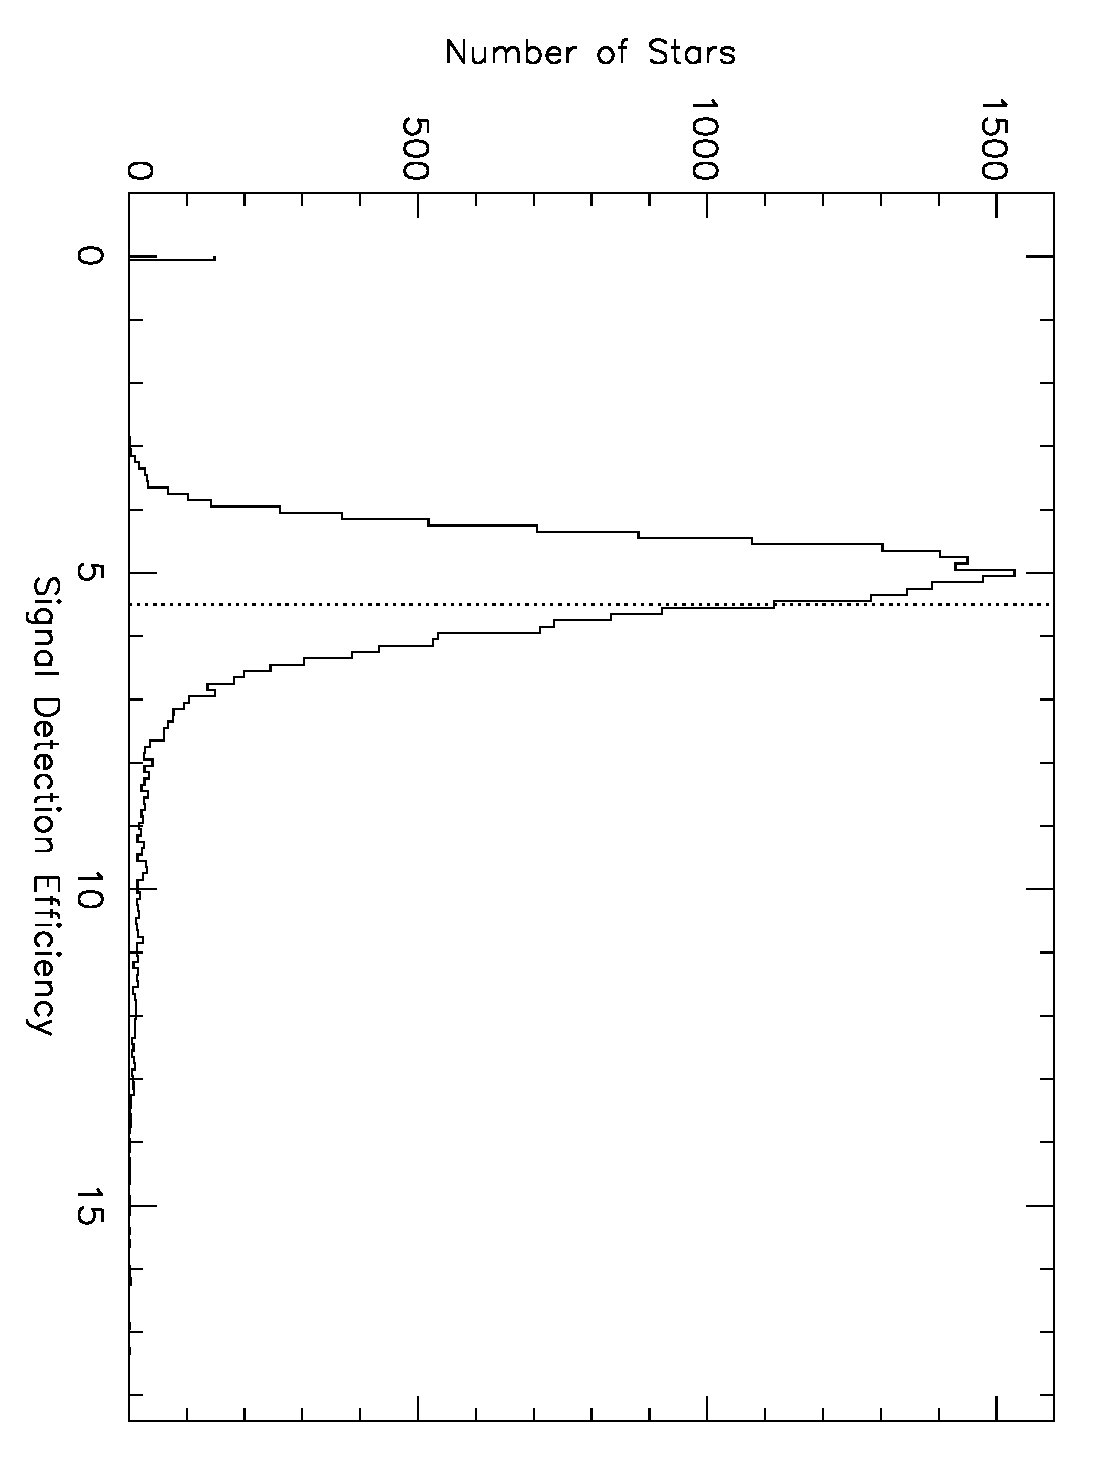
\includegraphics[width=.55\textwidth, angle=90]{7_sde_a}\\
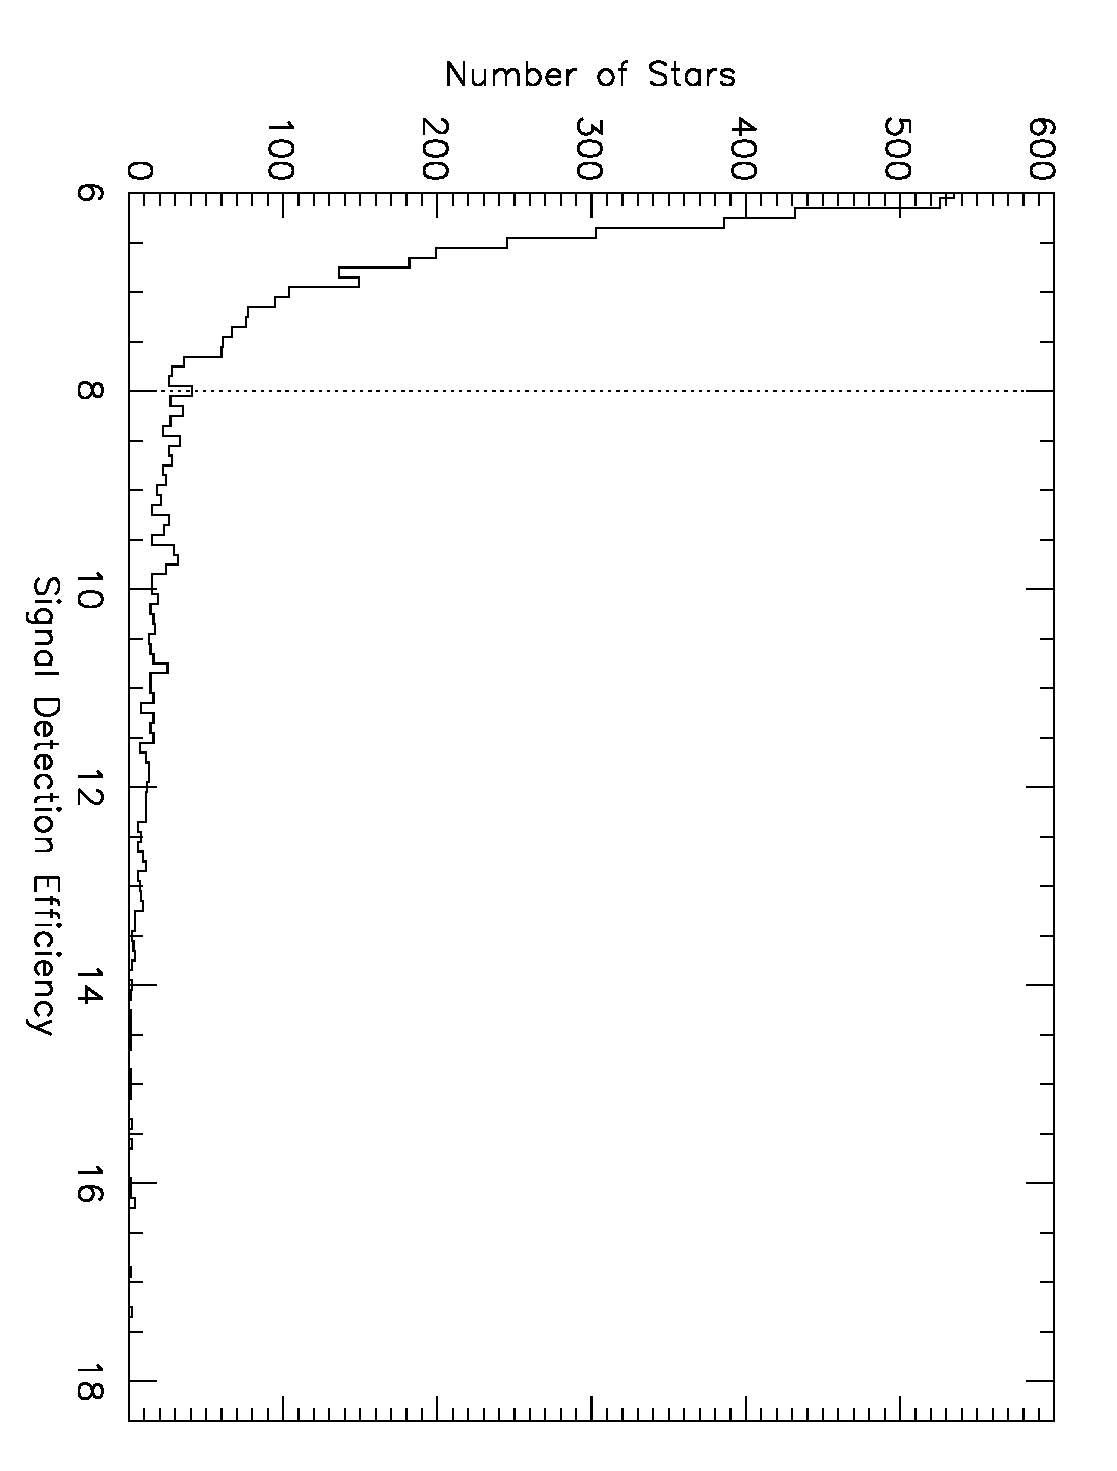
\includegraphics[width=.55\textwidth, angle=90]{7_sde_b}\\
\caption[Histograms of BLS SDEs for fake data set]{%
Histograms of the Signal Detection Efficiency (SDE) derived by the Box-fitting Least-Squares transit-search algorithm for: %
({\textit top panel}) the entire TrES Lyr1 data set with injected transits, and %
({\textit bottom panel}) those candidates with $\mathrm{SDE}\geq6$.
Saturated stars or stars with very noisy data were skipped by the algorithm, and assigned an SDE of 0.
The {\textit dotted} line in the {\textit top panel} denotes the minimum SDE of a candidate that will be visually inspected.
I first examined the candidates with SDEs to the right of the {\textit dotted} line in the {\textit bottom panel}, as they are more likely not to be spurious detections caused by random noise.
}\label{cha:human:sec:model:fig:sde}
\end{center}
\end{figure}


\begin{figure}
\begin{center}
\centering
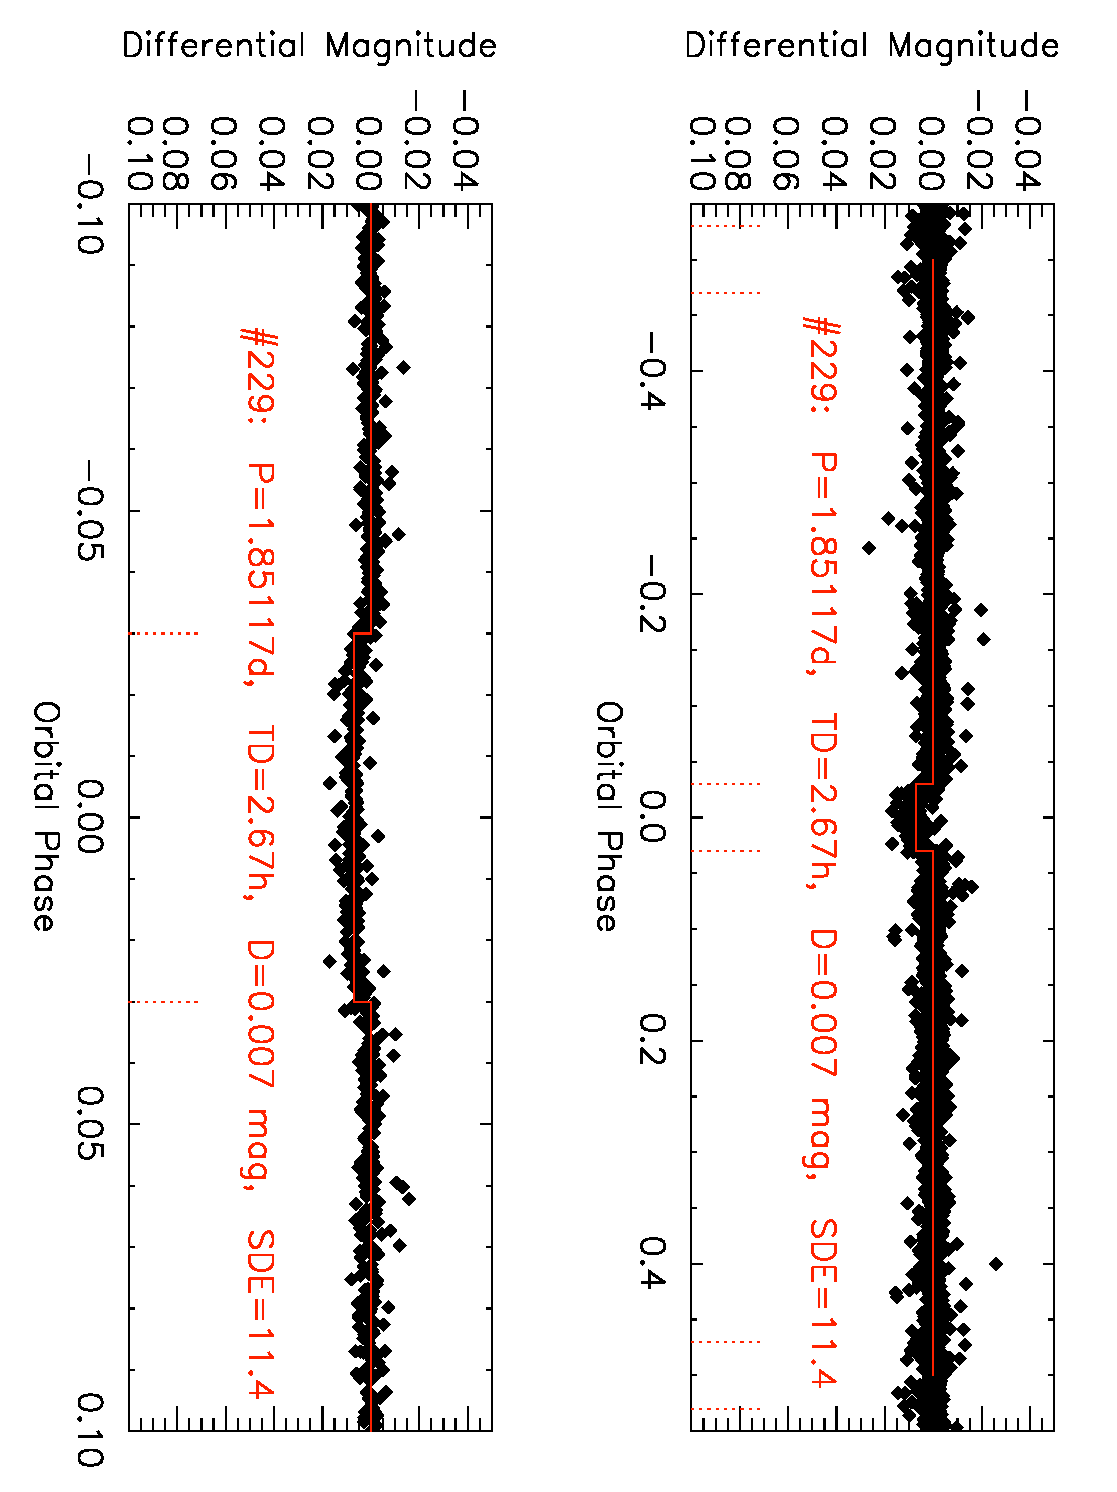
\includegraphics[width=.75\textwidth, angle=90]{7_highsde}
\caption[Example of an injected transit candidate with a high SDE]{%
Example of an injected transit candidate detected by the Box-fitting Least-Squares (BLS) algorithm with a high ($\geq$8) Signal Detection Efficiency (SDE).
Both plots show the variation in differential magnitude with orbital phase, and the four parameters (period P, duration TD, depth D, and SDE) output by the BLS algorithm are superimposed.
The {\textit upper} plot shows the entire orbit, whereas the {\textit lower} plot is at near-transit.
The {\textit dotted red lines} in both plots indicate (i) the point of ingress and egress of the box-transit (taken as $\pm d$, where $d$ is the BLS fractional duration), and (ii) this region shifted by 0.5 in phase to highlight the location where a secondary eclipse might be spotted.
I view plots similar to these for each transit candidate to determine the detection is real or spurious.%
}\label{cha:human:sec:model:fig:highsde}
\end{center}
\end{figure}

Treating the fake time series as a real data set from a TrES field, I then continued with the TrES procedure for identifying candidate transiting planets.
I searched the time series for periodic transit-like dips using the BLS algorithm, which assigns a Signal Detection Efficiency (SDE, see appendix~\ref{cha:bls}) statistic to each star based on the strength of the transit detection.
It represents a signal-to-noise ratio, where the signal is the average differential magnitude inside the transit compared to the average differential magnitude outside the transit, and the noise is the scatter of the differential magnitudes inside the transit.
I restricted my search to the period range (0.5--5\,days) and fractional duration range ($\sim$0.01--0.1) that I normally use for TrES data.
I restrict myself to periods less than 5\,days due to the necessity for a transit detection of observing multiple transits during an observing run, which typically lasts for TrES for about 40 clear nights.
The fractional duration range is based on what we would expect (\citealp*{Defay_Deleuil_Barge:aa:2001a}, and see figure~\ref{cha:human:sec:model:fig:bls2}) over a wide range of physical parameters, such as those chosen for this analysis, and for these orbital periods. Figure~\ref{cha:human:sec:model:fig:sde} shows a histogram of the derived SDEs for this fake data set.
From this figure, I chose $\mathrm{SDE}=8.0$ as a lower limit for my first visual examination, that of the candidates with the most significant detections.
Since there are few candidates with $\mathrm{SDE}\geq8.0$, I could concentrate on the best candidates without being overwhelmed by spurious transit light curves.
I then examined the candidates with $5.5 \leq \mathrm{SDE} < 8.0$ to find any remaining interesting candidates.
The lower limit here is taken to be just below the $\mathrm{SDE}=6$ limit that minimizes statistical false positives seen in \citet{Kovacs_Zucker_Mazeh:aa:2002a}.
Beyond this point, it will be difficult to find any true transit candidate, as the transit signal will be low and there will be many spurious transit light curves with similar SDEs.
Starting with the brightest stars, I examined each of the light curves with SDE$\geq8$, and then the light curves with $5.5<\mathrm{SDE}<8$.
I limited my search to candidates with $0.02 \leq (P\ \mathrm{mod}\ 0.5\,\mathrm{days})\leq 0.48$ and 0.004\,mmag $\leq \Delta \leq 0.1$\,mmag.
This limit avoids spurious detections with both integer or half-integer periods that are caused by a few bad data points within the supposed transit. Figure~\ref{cha:human:sec:model:fig:highsde} is an example of a plot of a high SDE candidate that I examined.

\section{BLS and Visual-Recovery Rates}\label{cha:human:sec:recrates}

The visual recovery of a transit light curve is heavily dependent on the accuracy of BLS transit parameters used to produce a phased light curve for inspection.
Therefore, as a first step in determining my ability to recover the fake transit light curve, I examined the recovery rate of injected transits for the BLS transit search.
The four parameters computed by BLS for each input light curve are the orbital period $P$ of the transits, the depth $\Delta$, the fractional duration $d$, and the orbital phase $\Phi$.
Of these, the most important is $P$.
As long as the light curve is correctly phased, I should be able to visually identify the transit.
Although the parameters $\Delta$, $d$, and $\Phi$ are used to overlay a model box-transit light curve and aid visual recovery, transit recovery is still possible if these parameters are highly inaccurate.
From experiments with several light curves where I varied the period used to phase the light curve while maintaining a visible transit signal, I chose the first recovery criterion to be that the derived orbital period is within 0.1\% of the true value.
The second criterion is that the derived transit ``depth'' is not negative.
This is because a transit light curve with a negative ``depth'' is automatically skipped by the code used to plot the transit candidates.

\begin{figure}
\begin{center}
\centering
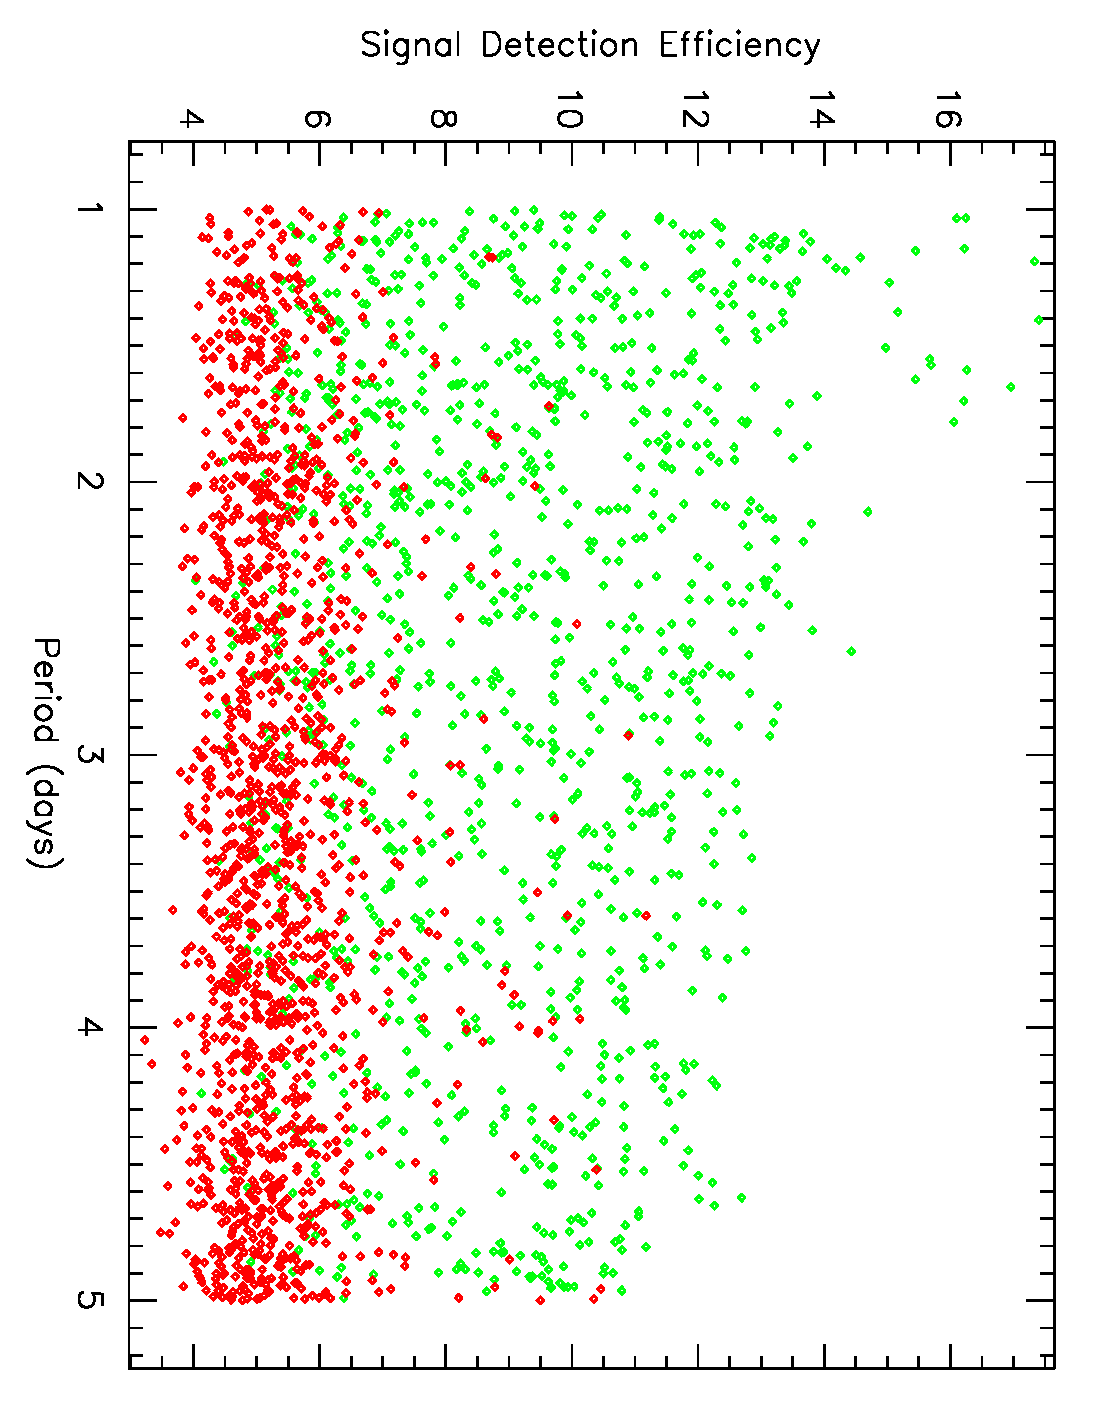
\includegraphics[width=.55\textwidth, angle=90]{7_comp_b} \\
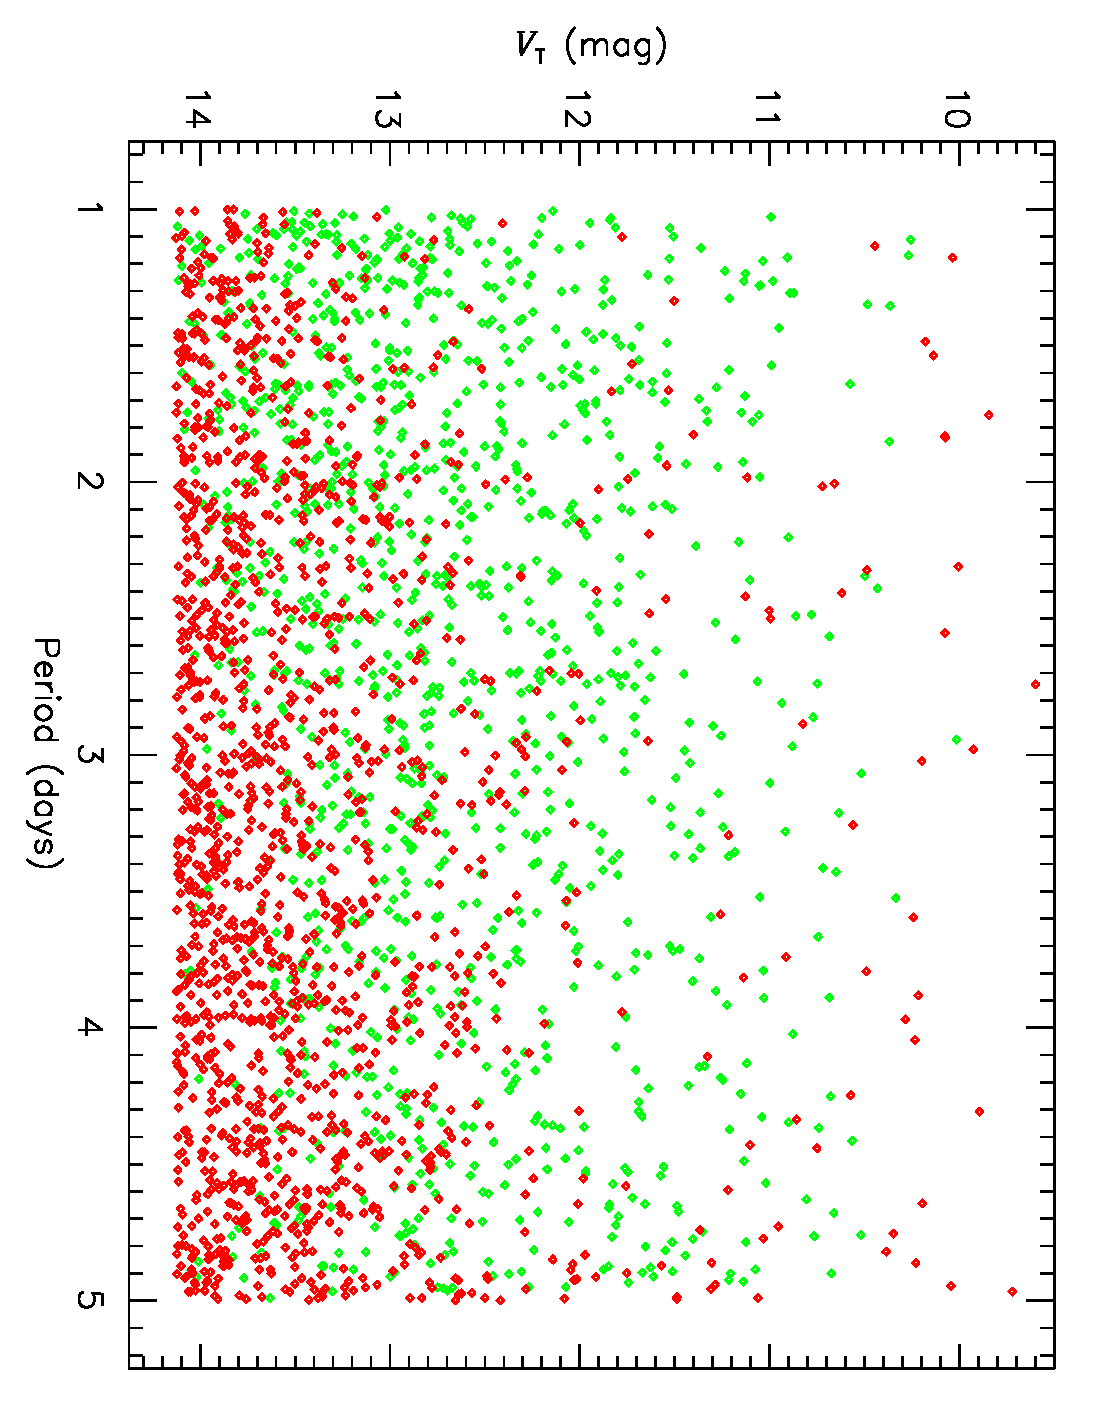
\includegraphics[width=.55\textwidth, angle=90]{7_comp_a} \\
\caption[SDE and $V_{T}$ versus period for BLS-recovered transits]{%
({\textit Top}) Signal Detection Efficiencies (SDEs) of the injected transit candidates plotted against their orbital period.
The candidates marked in {\textit green} were recovered by the Box-fitting Least-Squares (BLS) algorithm; that is, the derived orbital period was accurate to within 0.1\% and the transit depth was not negative.
{\textit Red diamonds} signify candidates not recovered by BLS.
BLS recovered the majority (79\%) of injected transit candidates with $\mathrm{SDE}\gsim6$.
({\textit Bottom}) Approximate $V_{T}$ magnitudes versus orbital period for the injected transit candidates.
BLS recovered 62\% of candidates with $V\leq13.5$\,mag.%
}\label{cha:human:sec:model:fig:rec}
\end{center}
\end{figure}

\begin{figure}
\begin{center}
\centering
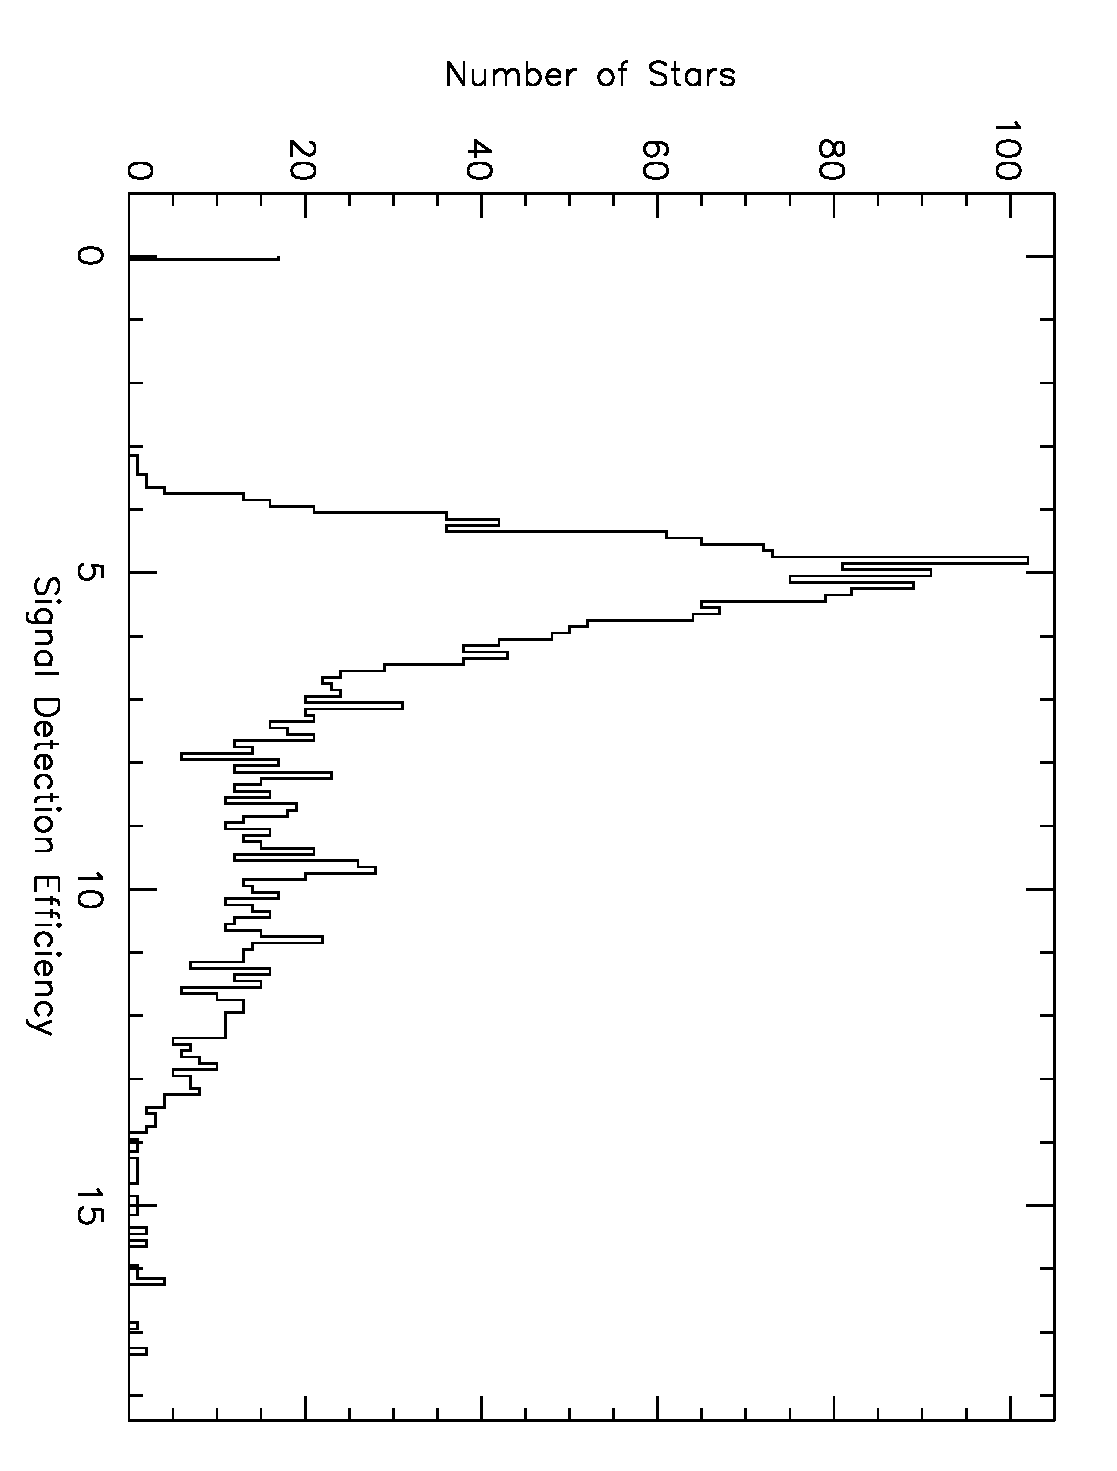
\includegraphics[width=.75\textwidth, angle=90]{7_comp_f}
\caption[Histogram of SDEs for BLS-recovered transit candidates]{%
Histogram of the Signal Detection Efficiency (SDE) derived by the Box-fitting Least-Squares transit-search algorithm for the injected transit candidates.%
}\label{cha:human:sec:model:fig:histsderec}
\end{center}
\end{figure}
\begin{figure}
\begin{center}
\centering
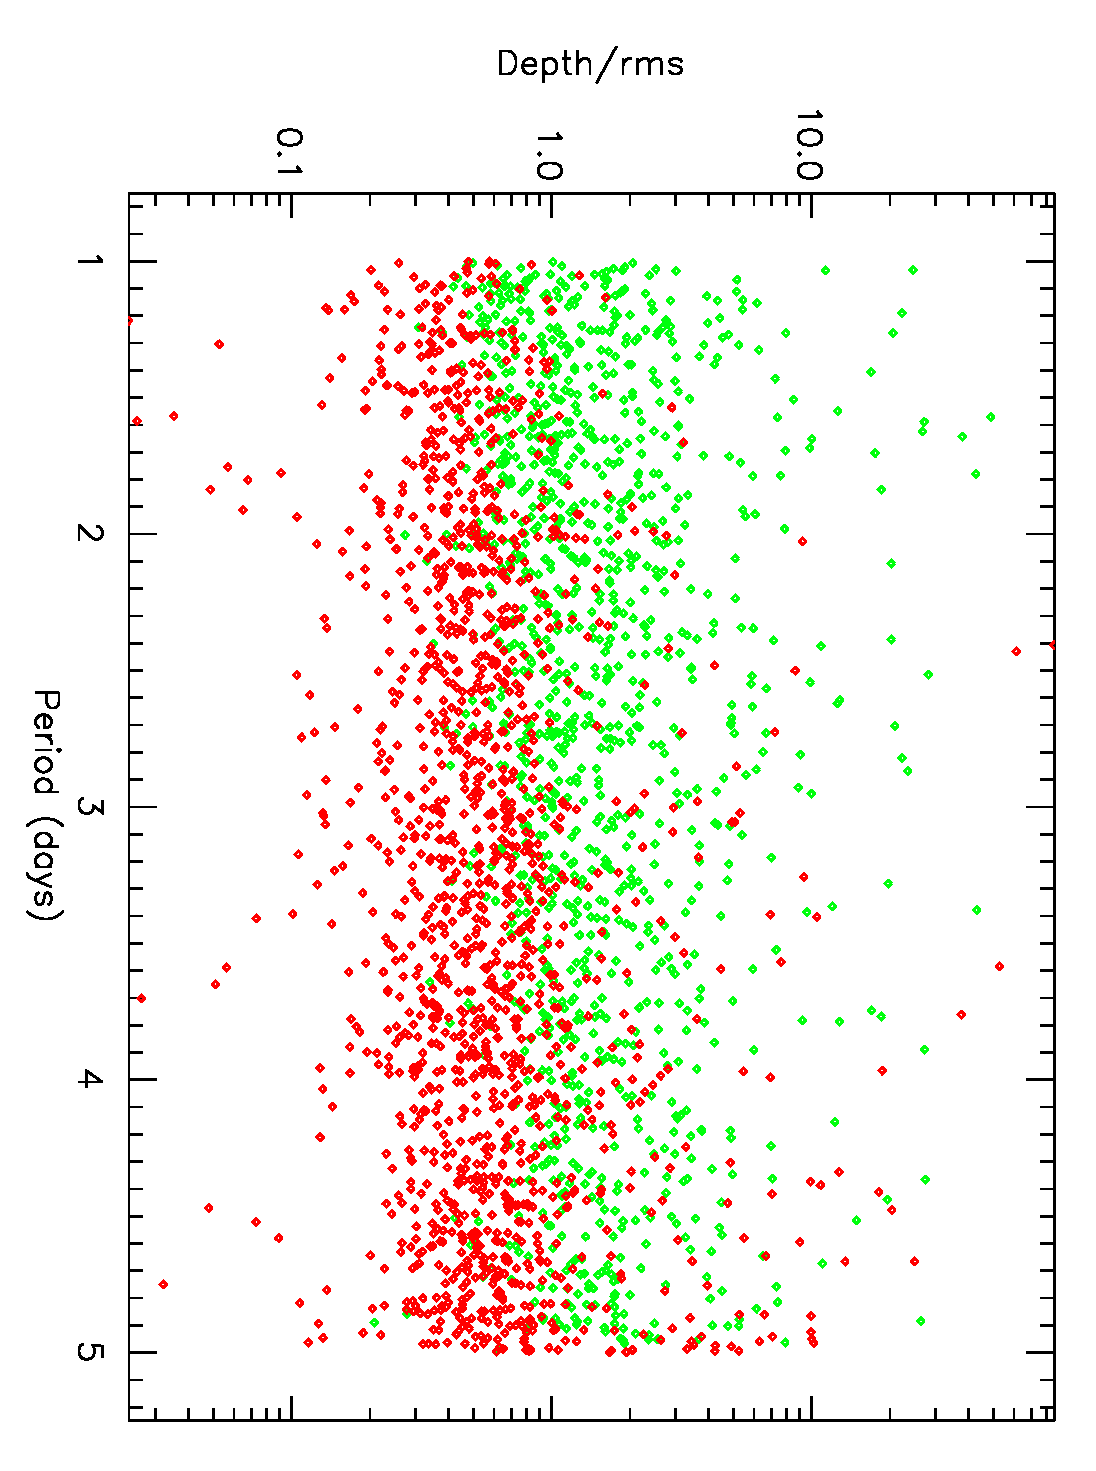
\includegraphics[width=.75\textwidth, angle=90]{7_comp_c} \\
\caption[Ratio of $\Delta$ to $\sigma$ versus period for BLS-recovered transits]{%
Same as figure~\ref{cha:human:sec:model:fig:rec}, but for the ratio of the transit depth ($\Delta$) to the rms ($\sigma$) of the TrES photometry.
Of the candidates with $\Delta\gsim\sigma$, 77\% were recovered by the transit-search algorithm (marked in {\textit green}; the candidates not recovered are in {\textit red}).%
}\label{cha:human:sec:model:fig:ratiorec}
\end{center}
\end{figure}

Of the 2,612 injected transit candidates, 1,153 were recovered by the BLS transit-search algorithm.
figure~\ref{cha:human:sec:model:fig:rec} %
shows the SDEs of these fake candidates, where the candidates in {\textit green} were recovered by the BLS algorithm and those in {\textit red} were not.
(A histogram of these SDEs for comparison with figure~\ref{cha:human:sec:model:fig:sde} can be seen in figure~\ref{cha:human:sec:model:fig:histsderec}.)
As can be clearly seen, the transit-search algorithm recovered the majority (79\%) of candidates with $\mathrm{SDE} \gsim 6$ but few with $\mathrm{SDE} < 6$. The latter are not significant detections \citep[see][]{Kovacs_Zucker_Mazeh:aa:2002a}.
The BLS recovery of candidates in terms of the magnitudes of the host star can also be seen in figure~\ref{cha:human:sec:model:fig:rec}%
.
Here the TrES instrumental $r$-band magnitude has been converted to an approximate Tycho-2 \citep{Hog_Fabricius_Makarov:aa:2000a} $V_{T}$ magnitude using the field stars with known $V_{T}$.
Again, the BLS algorithm recovers the majority (62\%) of transit candidates with $V_{T}\lsim 13.5$\,mag, except for the brighter, saturated stars.
These results can be better understood by comparing the transit depth to the rms ($\sigma$) of the photometry for the host star, as shown in figure~\ref{cha:human:sec:model:fig:ratiorec}. Of the transit candidates with $\Delta \gsim \sigma$,  77\% are recovered, with a slight bias against longer periods.

This suggests that $V_{T}\lsim 13.5$\,mag and $\Delta \gsim \sigma$ are the limits for the BLS algorithm as applied to TrES data.
Of the 1,459 candidates not recovered by the BLS algorithm, 1,197 had $\mathrm{SDE} < 6$, 868 had $V_{T}> 13.5$\,mag, and 1,230 had $\Delta < \sigma$. When these factors are taken into account, only 39 (1\%) candidate transit signals that we would expected the algorithm to detect were not recovered.

\begin{figure}
\begin{center}
\centering
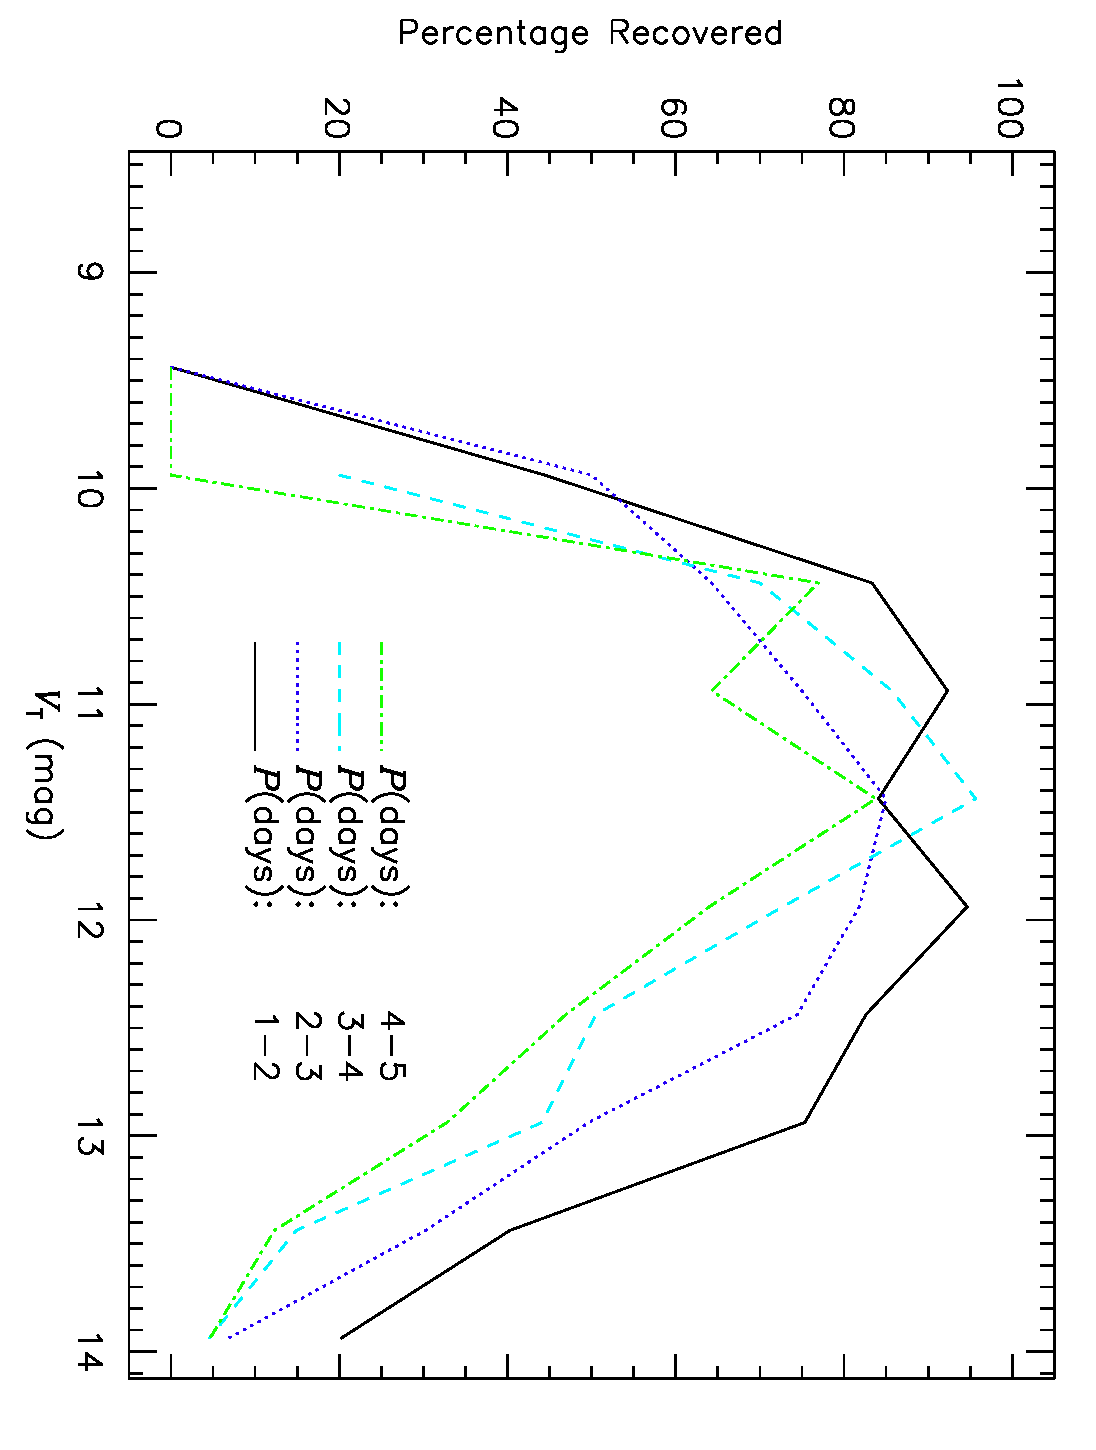
\includegraphics[width=.55\textwidth, angle=90]{7_comp_d}\\
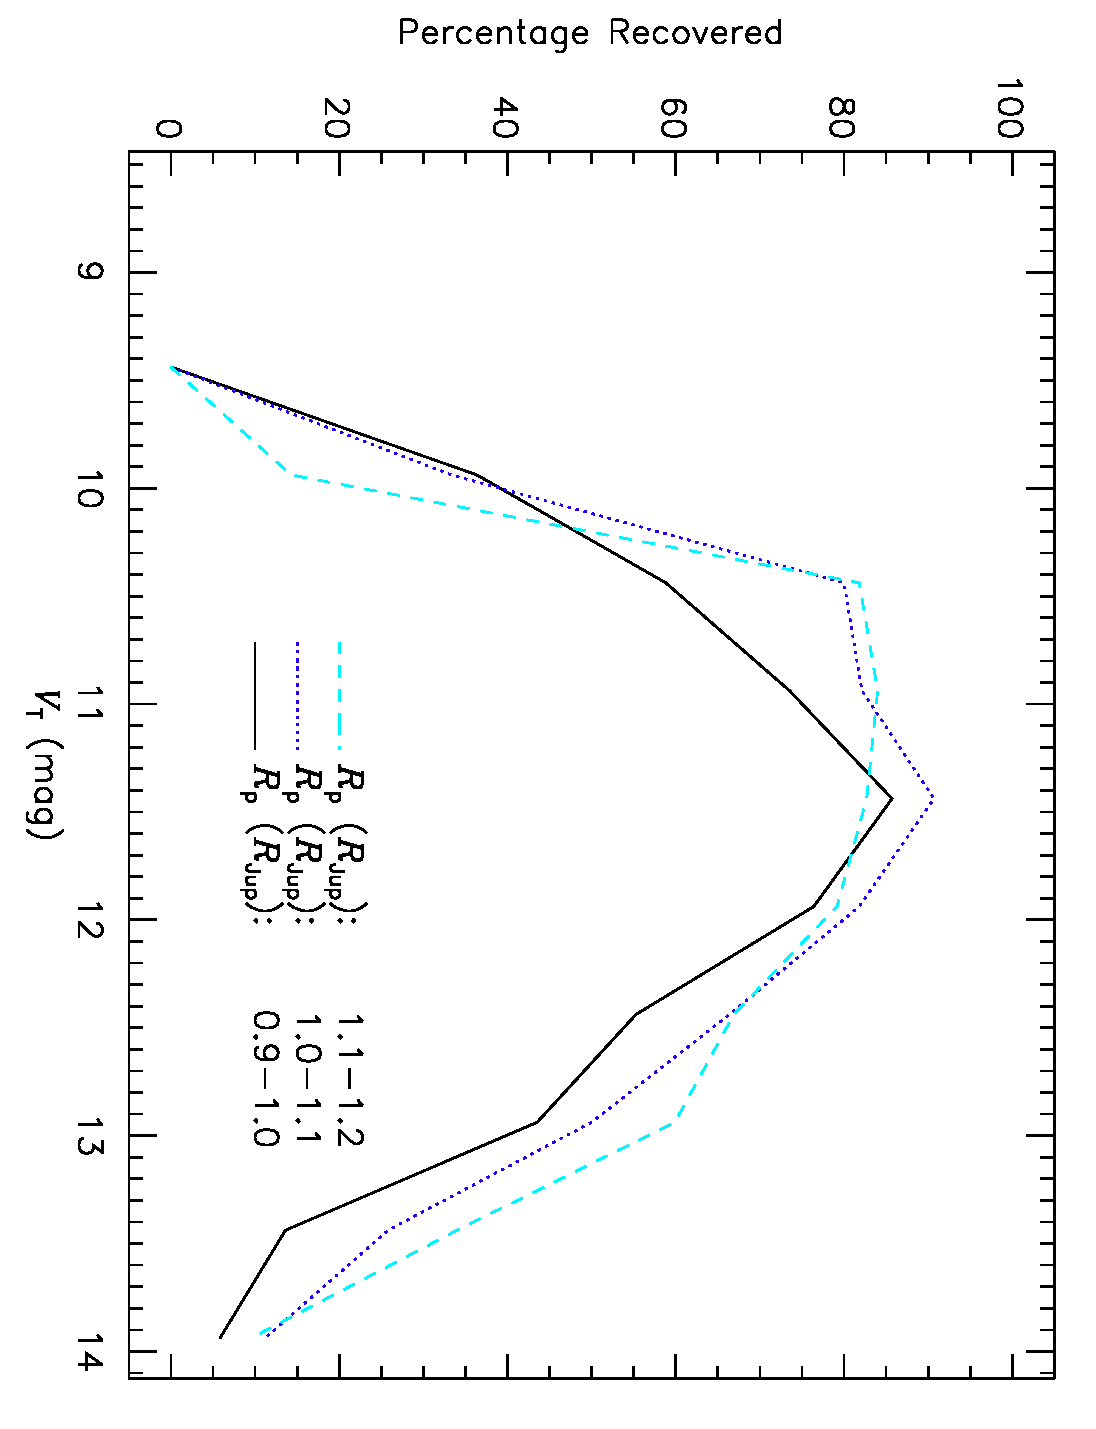
\includegraphics[width=.55\textwidth, angle=90]{7_comp_e}\\
\caption[BLS recovery rates for different orbital periods and planetary radii]{%
Percentage of the injected transit candidates recovered by the automated BLS transit-search algorithm as a function of approximate $V_{T}$ magnitude for different ranges in: %
%($a$)
({\textit top panel}) orbital period $P$, and %
%($b$)
({\textit bottom panel}) planetary radii $R_{p}$. %
The recovery rates have been averaged in bins in $V_{T}$ of 0.5\,mag.%
}\label{cha:human:sec:model:fig:recrates1}
\end{center}
\end{figure}

\begin{figure}
\begin{center}
\centering
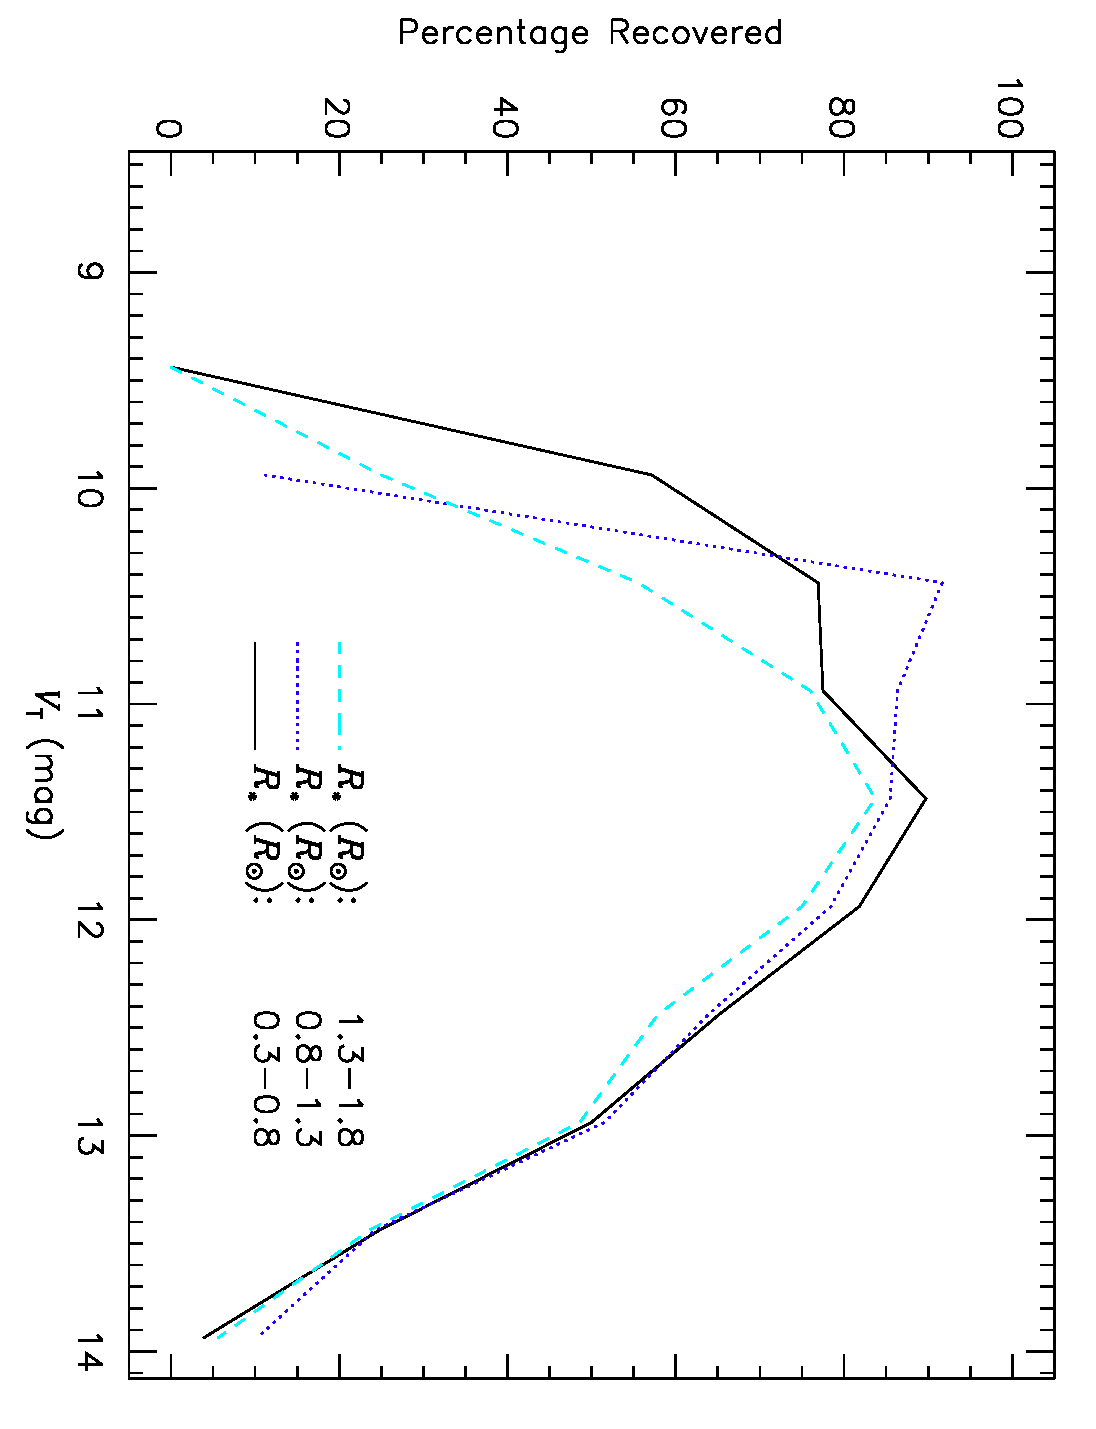
\includegraphics[width=.55\textwidth, angle=90]{7_comp_h}\\
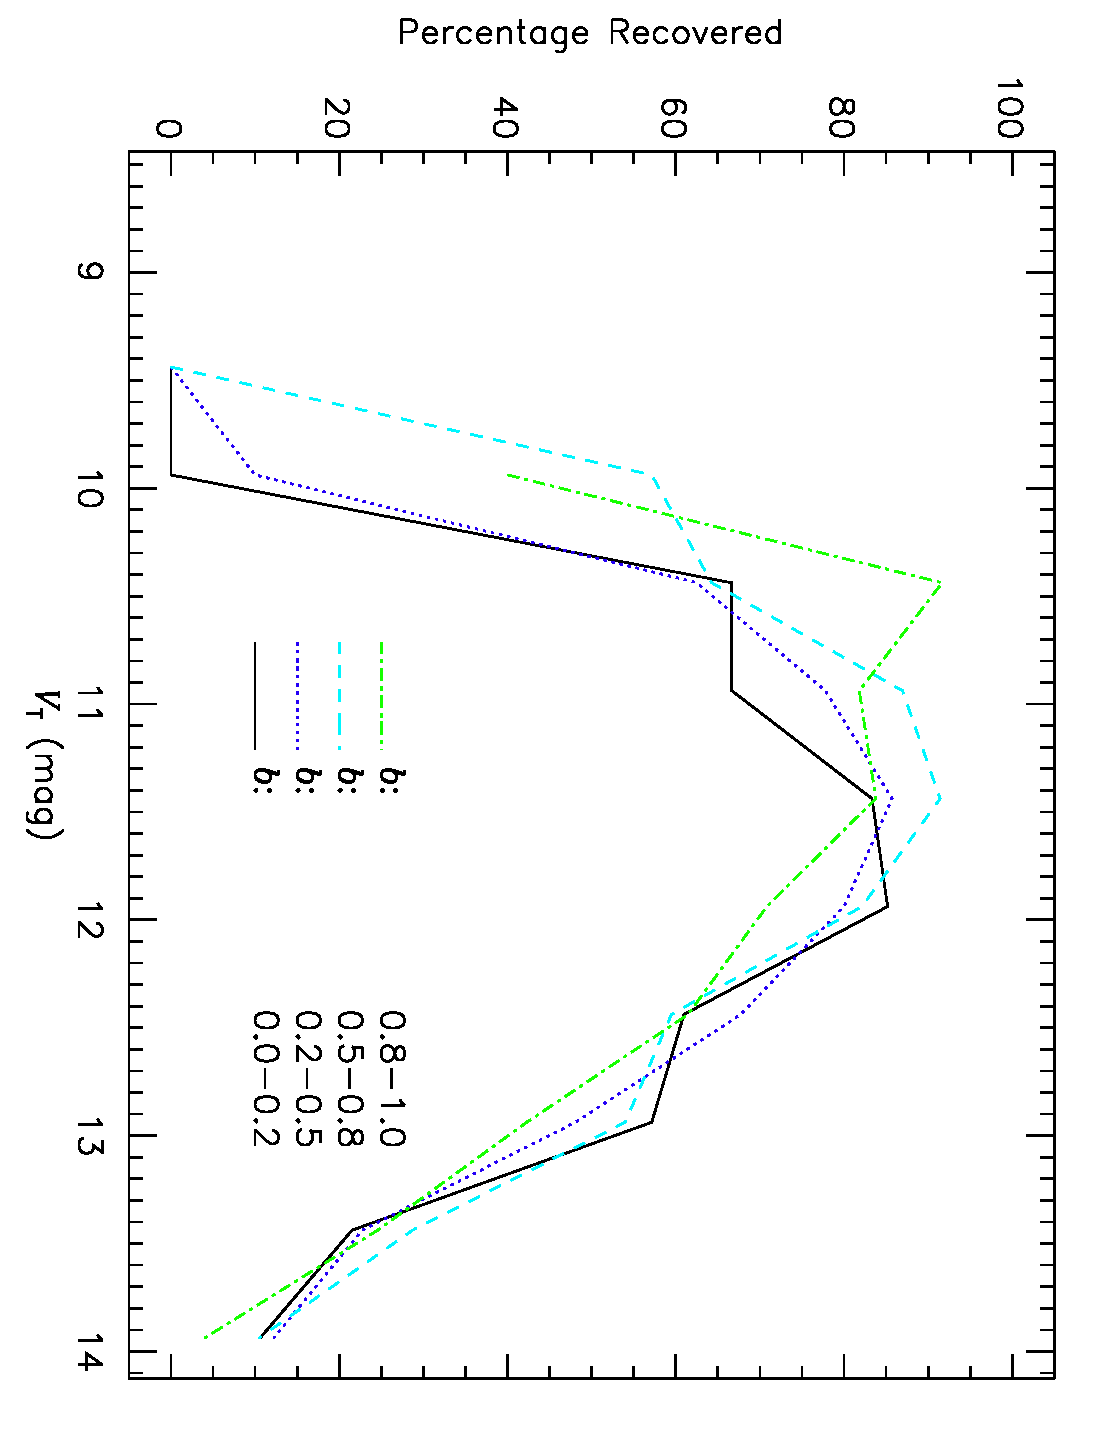
\includegraphics[width=.55\textwidth, angle=90]{7_comp_i}\\
\caption[BLS recovery rates for different stellar radii and impact parameters]{%
Same as for figure~\ref{cha:human:sec:model:fig:recrates1}, but for: %
%($a$)
({\textit top panel})  stellar radii $R_{\star}$, and %
%($b$)
({\textit bottom panel})  impact parameters $b$. %
}\label{cha:human:sec:model:fig:recrates2}
\end{center}
\end{figure}

The variation of the recovery rate with stellar magnitude for different orbital periods, planetary radii, stellar radii and impact parameters is shown in figures~\ref{cha:human:sec:model:fig:recrates1} and~\ref{cha:human:sec:model:fig:recrates2}.
As would be expected, the recovery rates drop for the fainter stars ($V_{T}>$13.5 mag) and the brightest, saturated stars ($V_{T}<$10.0\,mag).
The rate also increases for shorter periods, larger planets, and smaller stars, although the trend is not robust due to the relatively small number of candidate transits.
This bias is not surprising, as a larger planet and smaller star increases $\Delta$, and a shorter period increases the number of observed transits. However, the rate does seem to increase slightly with larger impact parameters, which is surprising. A large impact parameter implies a V-shaped light curve indicative of an eclipsing binary, rather than the typical transit light curve.
Overall, the recovery rate for the BLS algorithm is about 80\% for the average magnitudes of $11 \leq V_{T} \leq 12$\,mag.

\begin{figure}
\begin{center}
\centering
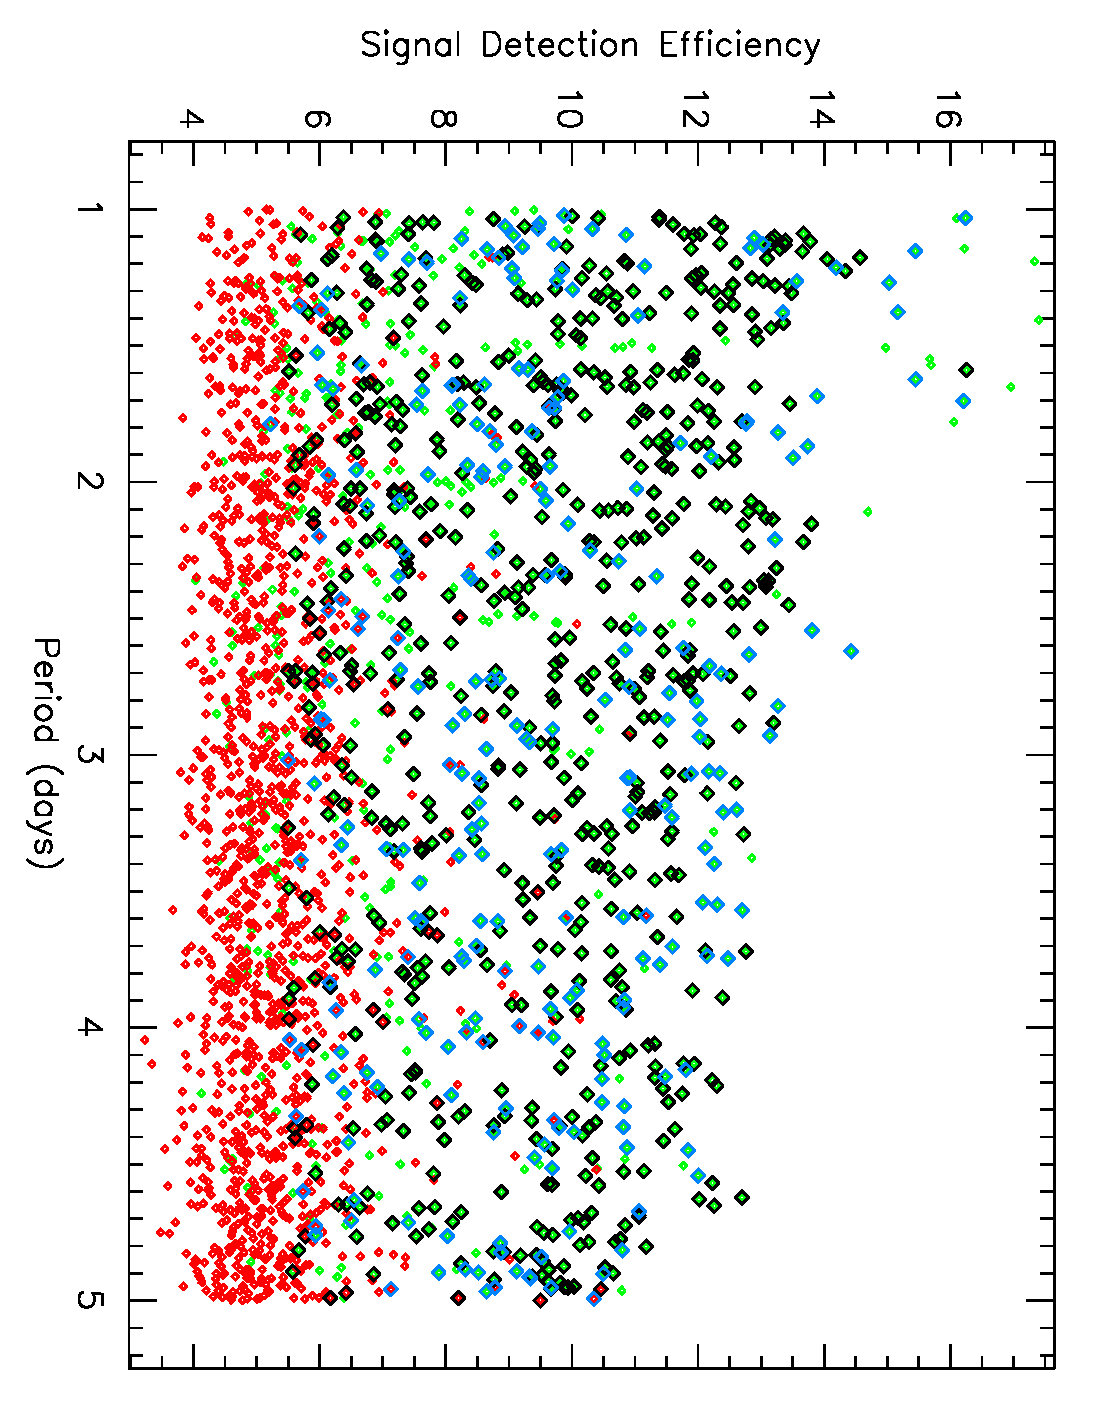
\includegraphics[width=.55\textwidth, angle=90]{7_visual_b} \\
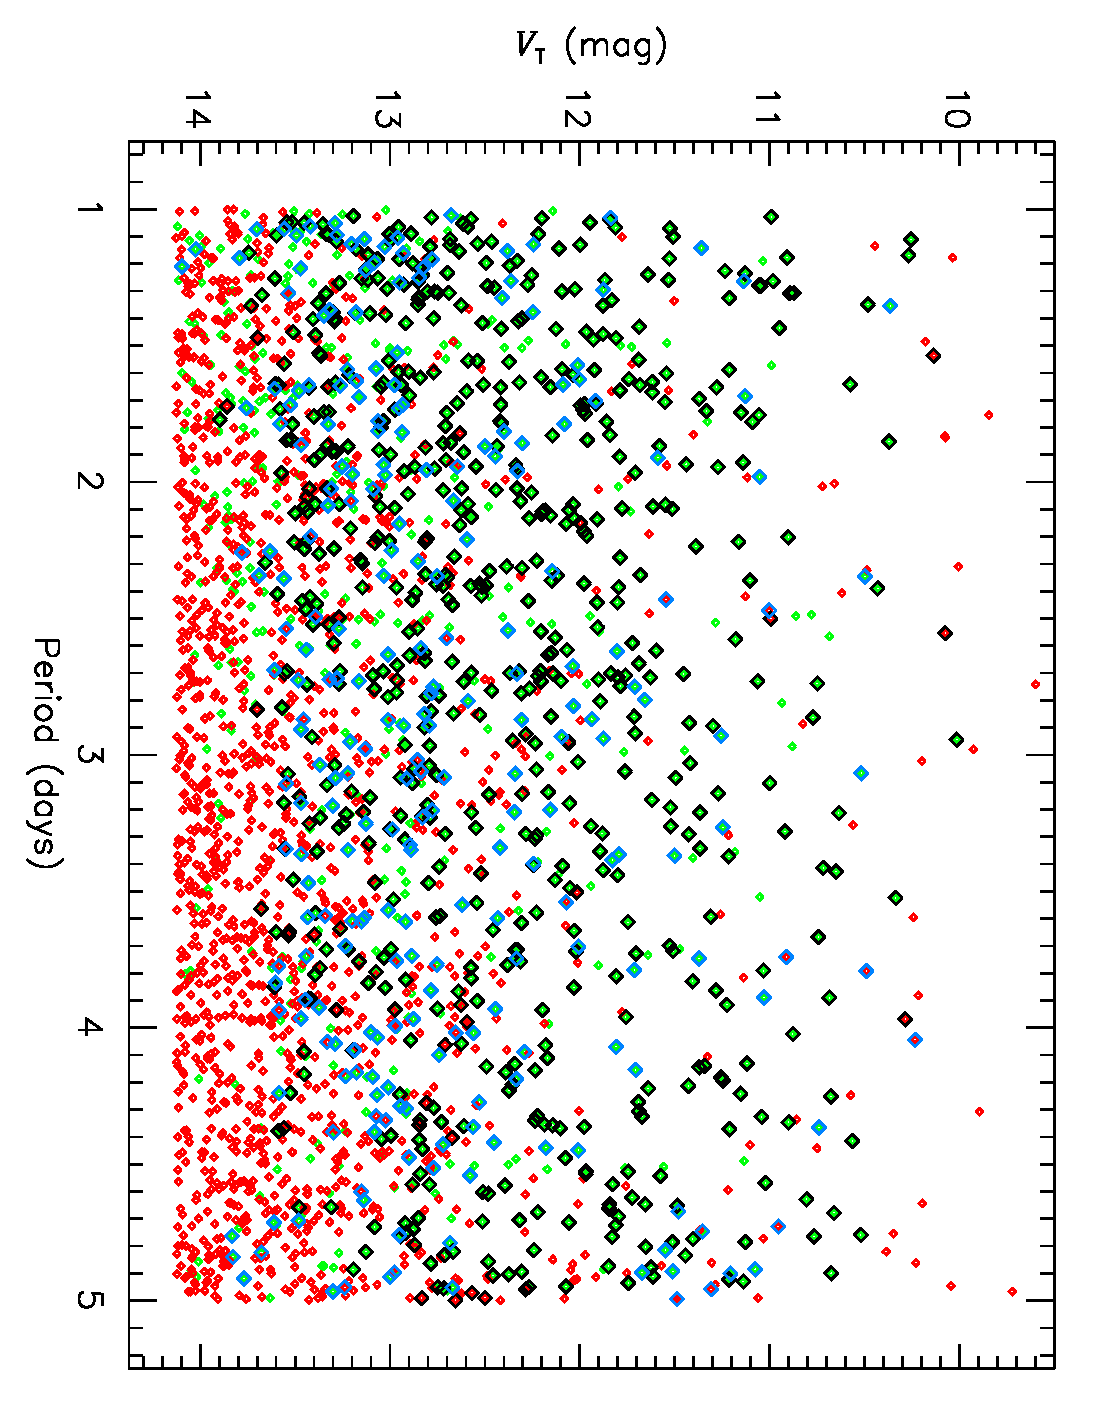
\includegraphics[width=.55\textwidth, angle=90]{7_visual_a} \\
\caption[SDE and $V_{T}$ versus period for visually recovered transits]{%
%($a$)
({\textit Top}) As for {\textit top panel} of figure~\ref{cha:human:sec:model:fig:rec}%$a$
, except that here the candidates outlined in {\textit black} were visually recovered, and those outlined in {\textit blue} were visually identified but discarded.
%($b$)
({\textit Bottom}) Same as the {\textit top panel}, but for approximate $V_{T}$ magnitudes versus orbital period for the injected transit candidates.%
}\label{cha:human:sec:model:fig:visrec}
\end{center}
\end{figure}

\begin{figure}
\begin{center}
\centering
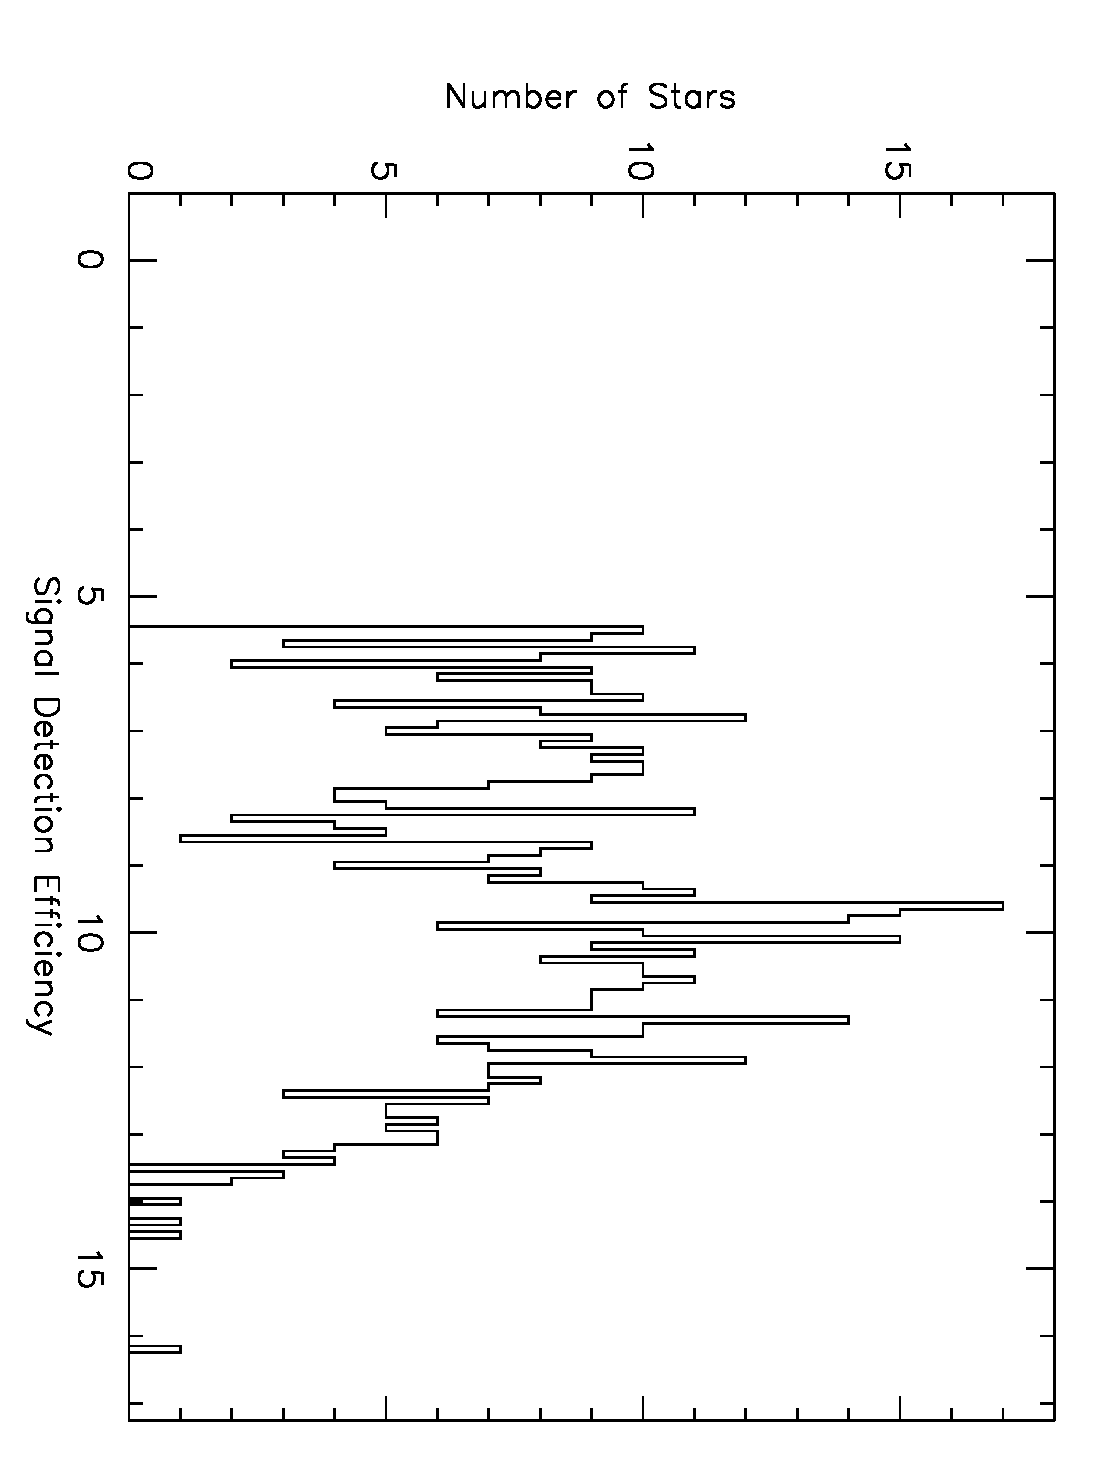
\includegraphics[width=.75\textwidth, angle=90]{7_visual_f}
\caption[Histogram of SDEs for visually recovered transit candidates]{%
Histogram of the Signal Detection Efficiency (SDE) derived by the Box-fitting Least-Squares transit-search algorithm for the injected transit candidates that were visually recovered.%
}\label{cha:human:sec:model:fig:vishistsderec}
\end{center}
\end{figure}

\begin{figure}
\begin{center}
\centering
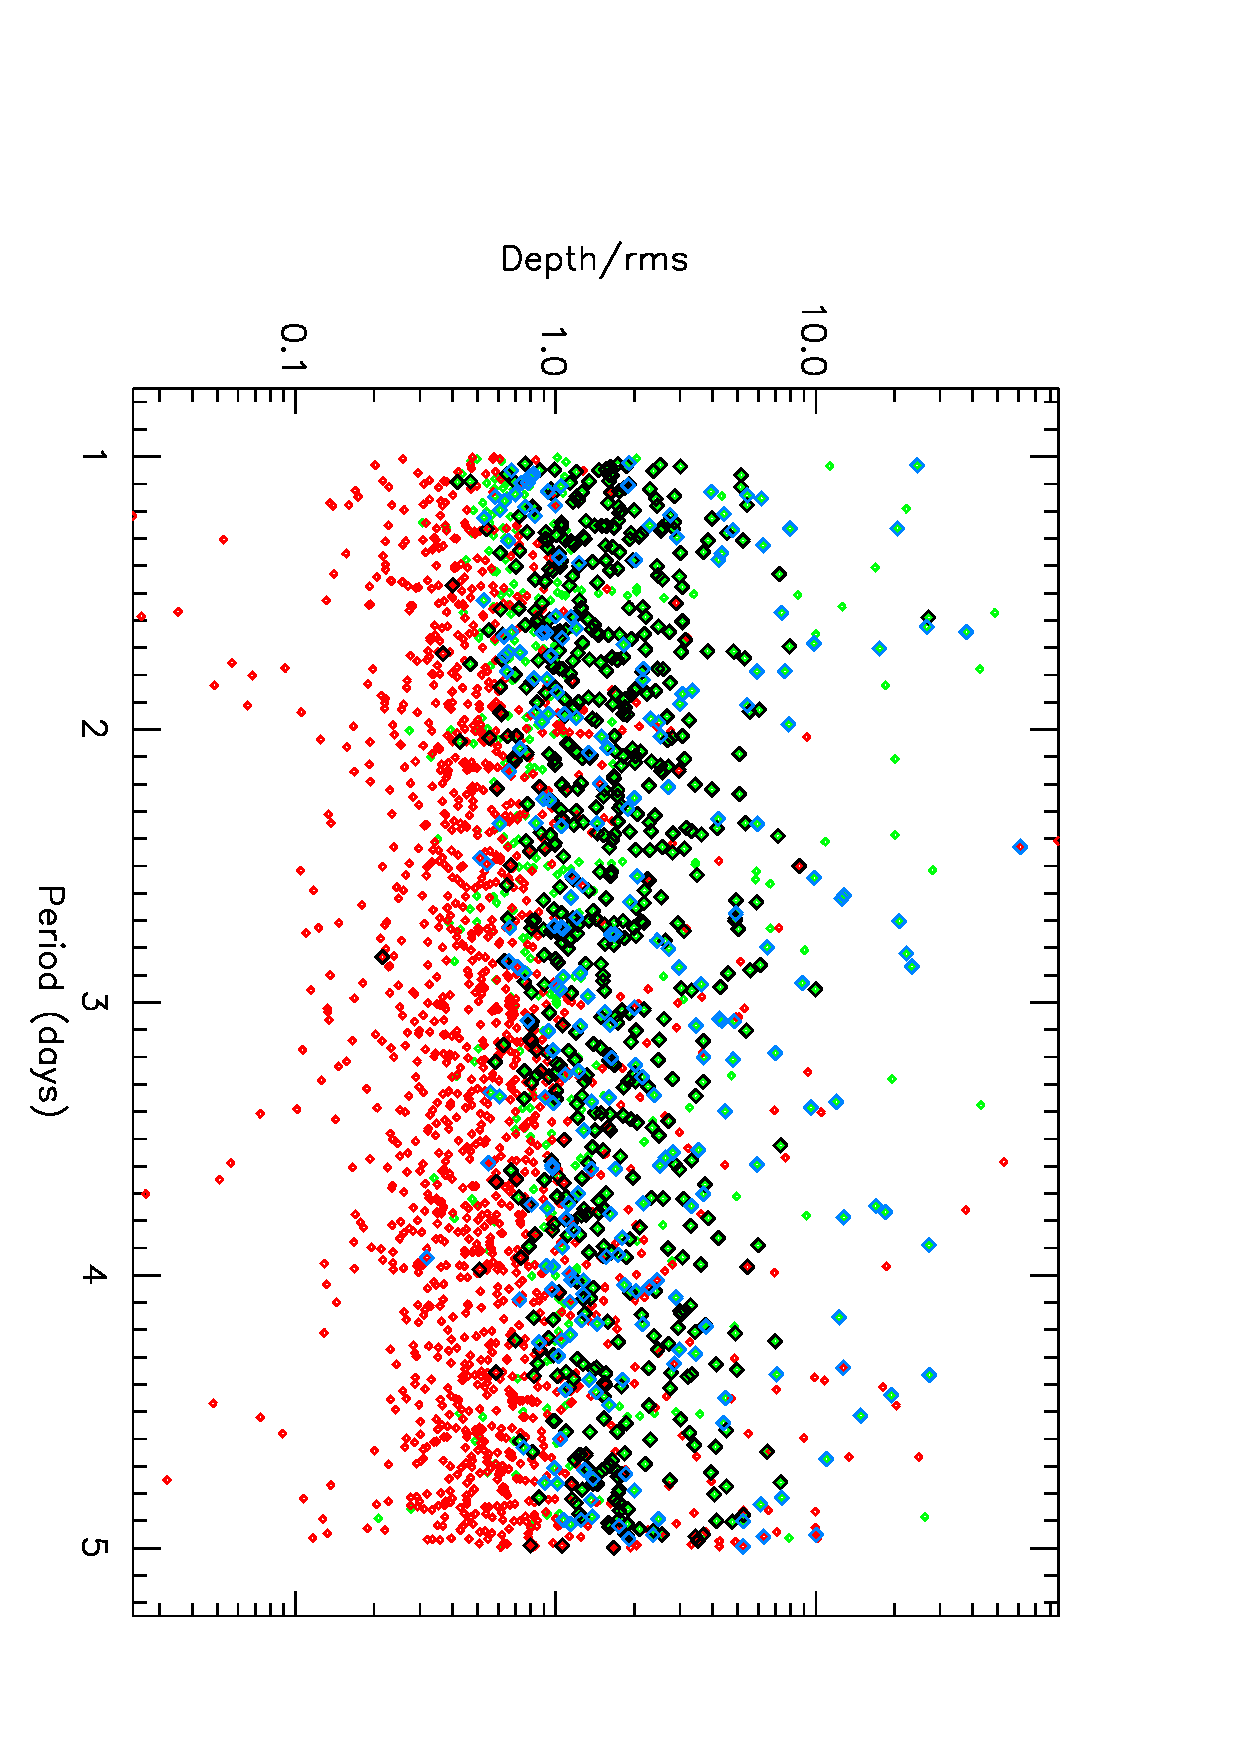
\includegraphics[width=.75\textwidth, angle=90]{7_visual_c} \\
\caption[$\Delta/\sigma$ versus period for visually recovered transits]{%
Same as figure~\ref{cha:human:sec:model:fig:visrec}, but for the ratio of the transit depth ($\Delta$) to the rms ($\sigma$) of the TrES photometry plotted versus the orbital period for the injected transit candidates.%
}\label{cha:human:sec:model:fig:visratiorec}
\end{center}
\end{figure}

Of the 2,612 injected transit candidates, I recovered 641 visually, compared to 1,153 recovered by the BLS algorithm.
I have reproduced the earlier plots showing the SDEs, magnitudes, and depth-to-rms ratios of the fake candidates in figures~\ref{cha:human:sec:model:fig:visrec}, \ref{cha:human:sec:model:fig:vishistsderec}, and~\ref{cha:human:sec:model:fig:visratiorec}. I have then outlined candidates that I visually recovered with a {\textit black diamond}, and those candidates that I visually recovered, but dismissed for some reason (such as poor phase coverage at transit, or a large depth more typical of an eclipsing binary), with a {\textit blue diamond.}
We can see that although I visually recovered many of the candidates, there are several candidates with large SDEs, bright magnitudes and high depth-to-rms ratios that I missed.
I also discarded several candidates with large SDEs.
We can also see that I recovered some of the candidates that failed my recovery test for the BLS algorithm, although I dismissed them as spurious.
I examined the properties of the BLS-recovered candidate transits that I did not visually identify or that I dismissed.
I found that 71\% were faint ($V_{T}>13.5$\,mag), and 52\% had a depth less than the scatter of the photometry.
This would indicate that I could not visually distinguish these signals from spurious detections in poor-quality photometry, despite the fact that these signals were recovered by the BLS algorithm.
About 20\% had periods or depths outside the limits of my transit plotting code, and hence were skipped and never viewed.
Although these limits were imposed to reduce the number of false detections due to bad data from a single night of observation, the resulting high fraction of missed transit signals suggests revisiting this step of my transit search.
Finally, 25\% of the candidates that I would not have pursued had depths greater than 0.03\,mag.
figure~\ref{cha:human:sec:model:fig:bls1} %$b$
shows how relatively few transits with such large depths would be expected in a field survey such as ours.
Our early experience with pursuing such candidates has reinforced their poor return, and we normally do not consider them a worthwhile investment.
Having accounted for all but 12\% (82) of the transit candidates that I did not visually recover, I examined the light curves of the remaining candidates with an $\mathrm{SDE}\geq8$.
I confirmed that for all but a few I rejected the transit light curve as having few data points within the transit.


\begin{figure}
\begin{center}
\centering
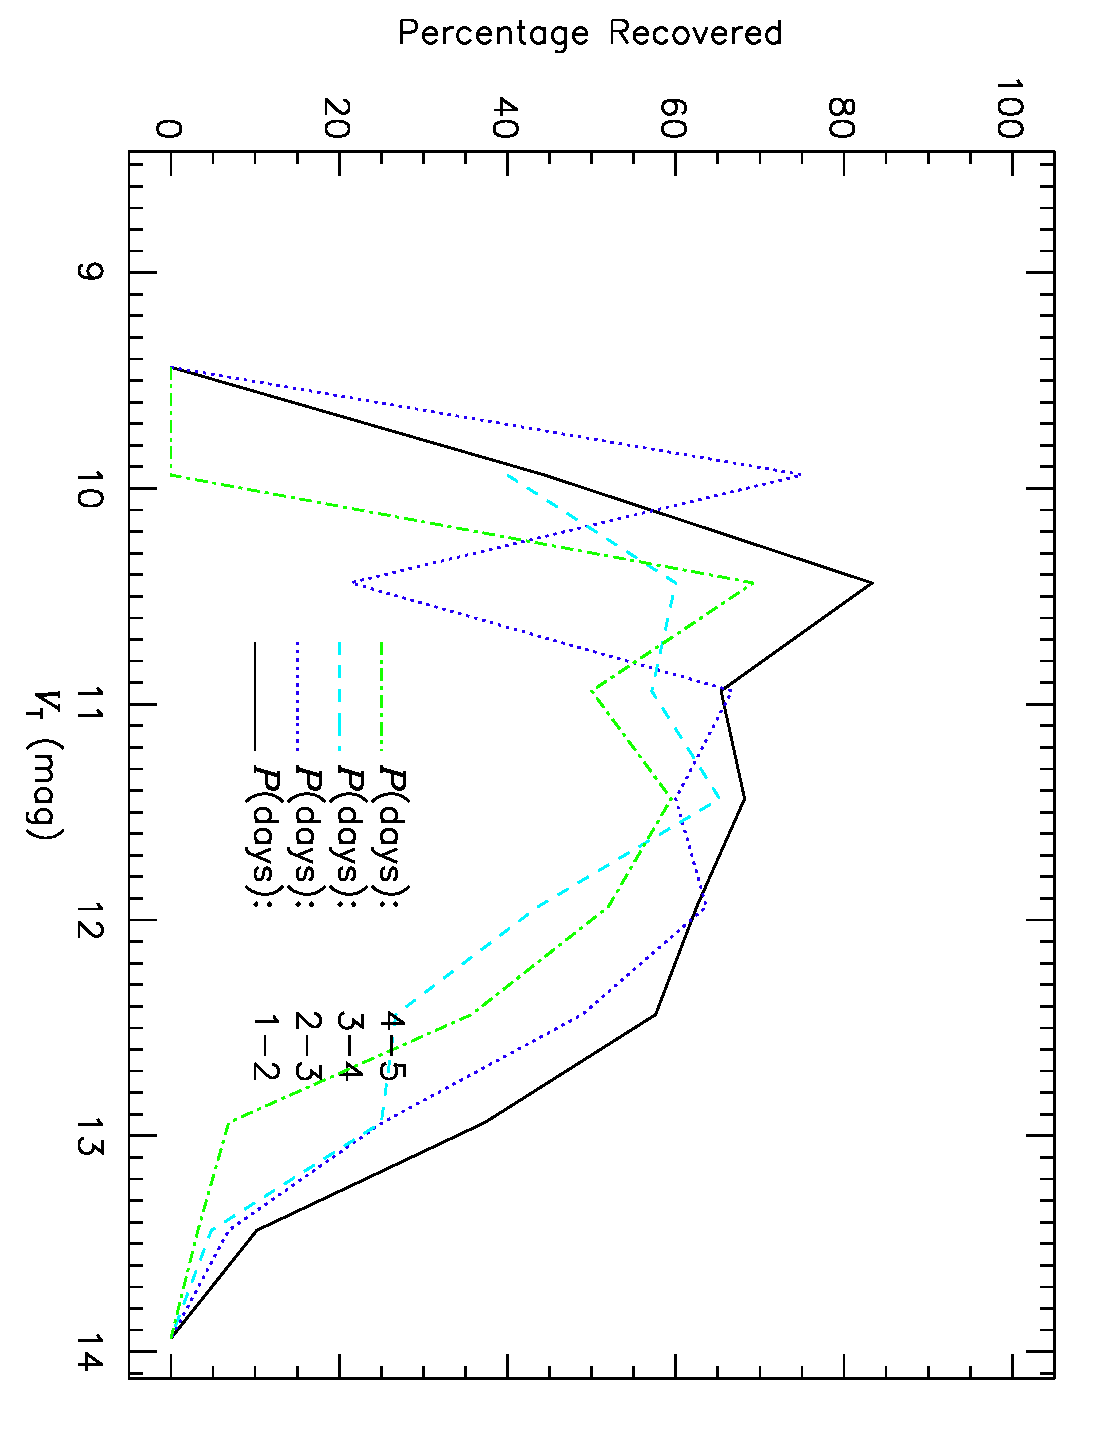
\includegraphics[width=.55\textwidth, angle=90]{7_visual_d}\\
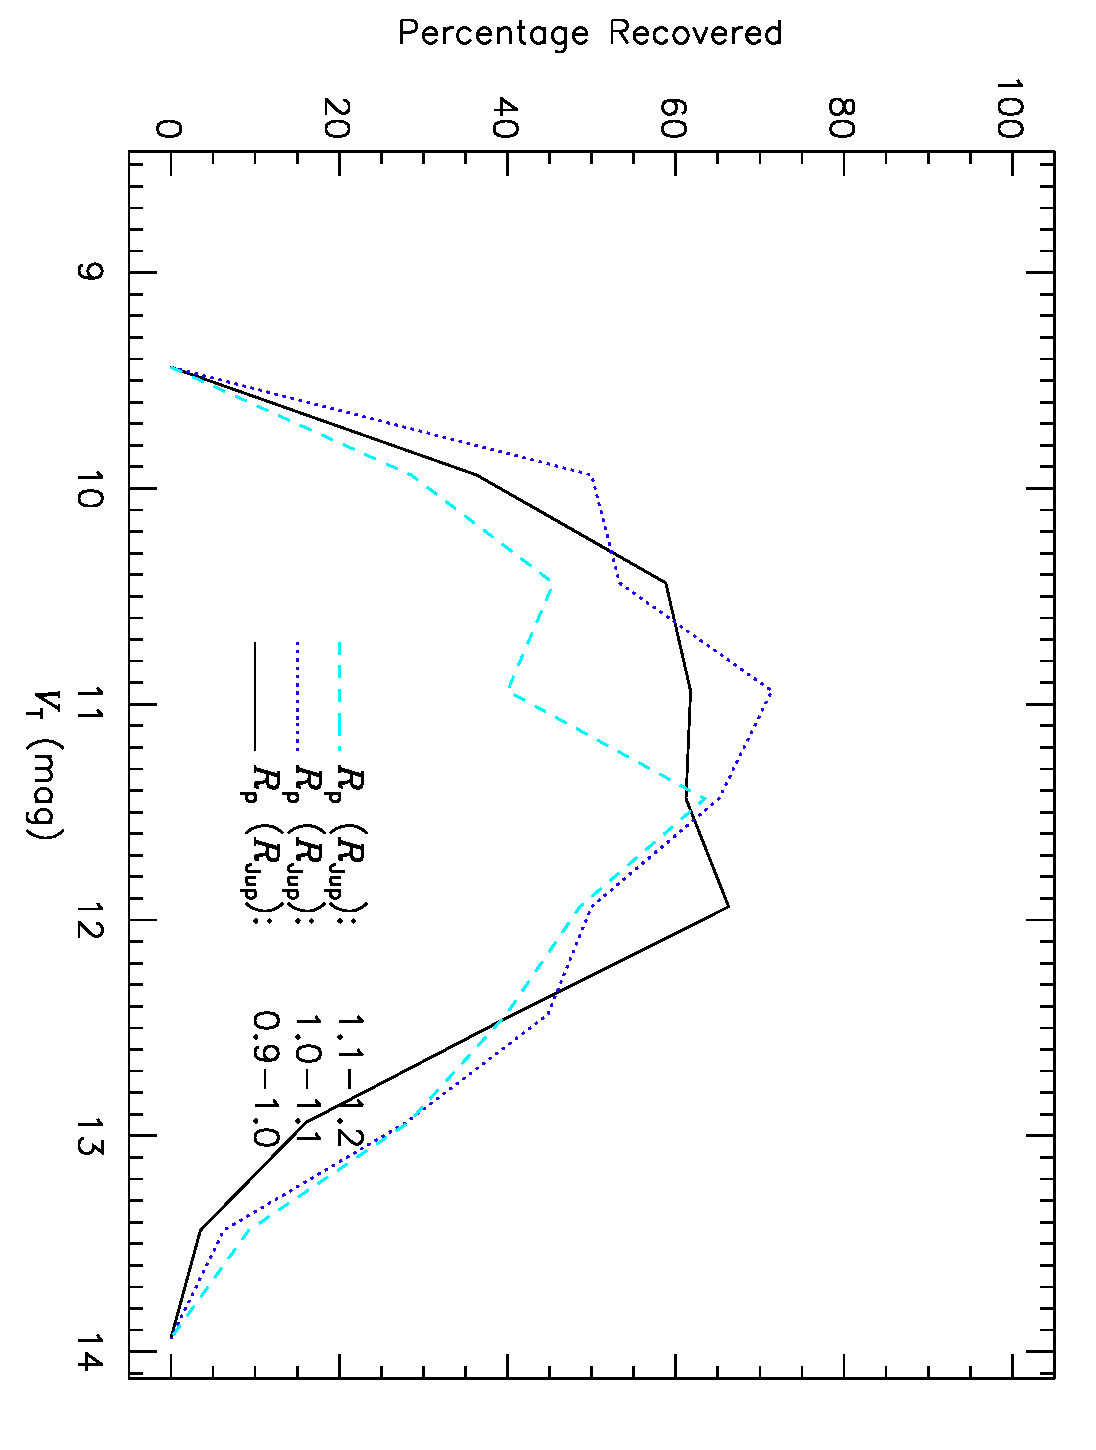
\includegraphics[width=.55\textwidth, angle=90]{7_visual_e}\\
\caption[Visual-recovery rates for different periods and planetary radii]{%
Percentage of the injected transit candidates visually recovered as a function of approximate $V_{T}$ magnitude for different ranges in: %
%($a$)
({\textit top panel}) orbital period $P$, and %
%($b$)
({\textit bottom panel}) planetary radii $R_{p}$. %
The recovery rates have been averaged in bins in $V_{T}$ of 0.5\,mag.%
}\label{cha:human:sec:model:fig:visrecrates1}
\end{center}
\end{figure}

\begin{figure}
\begin{center}
\centering
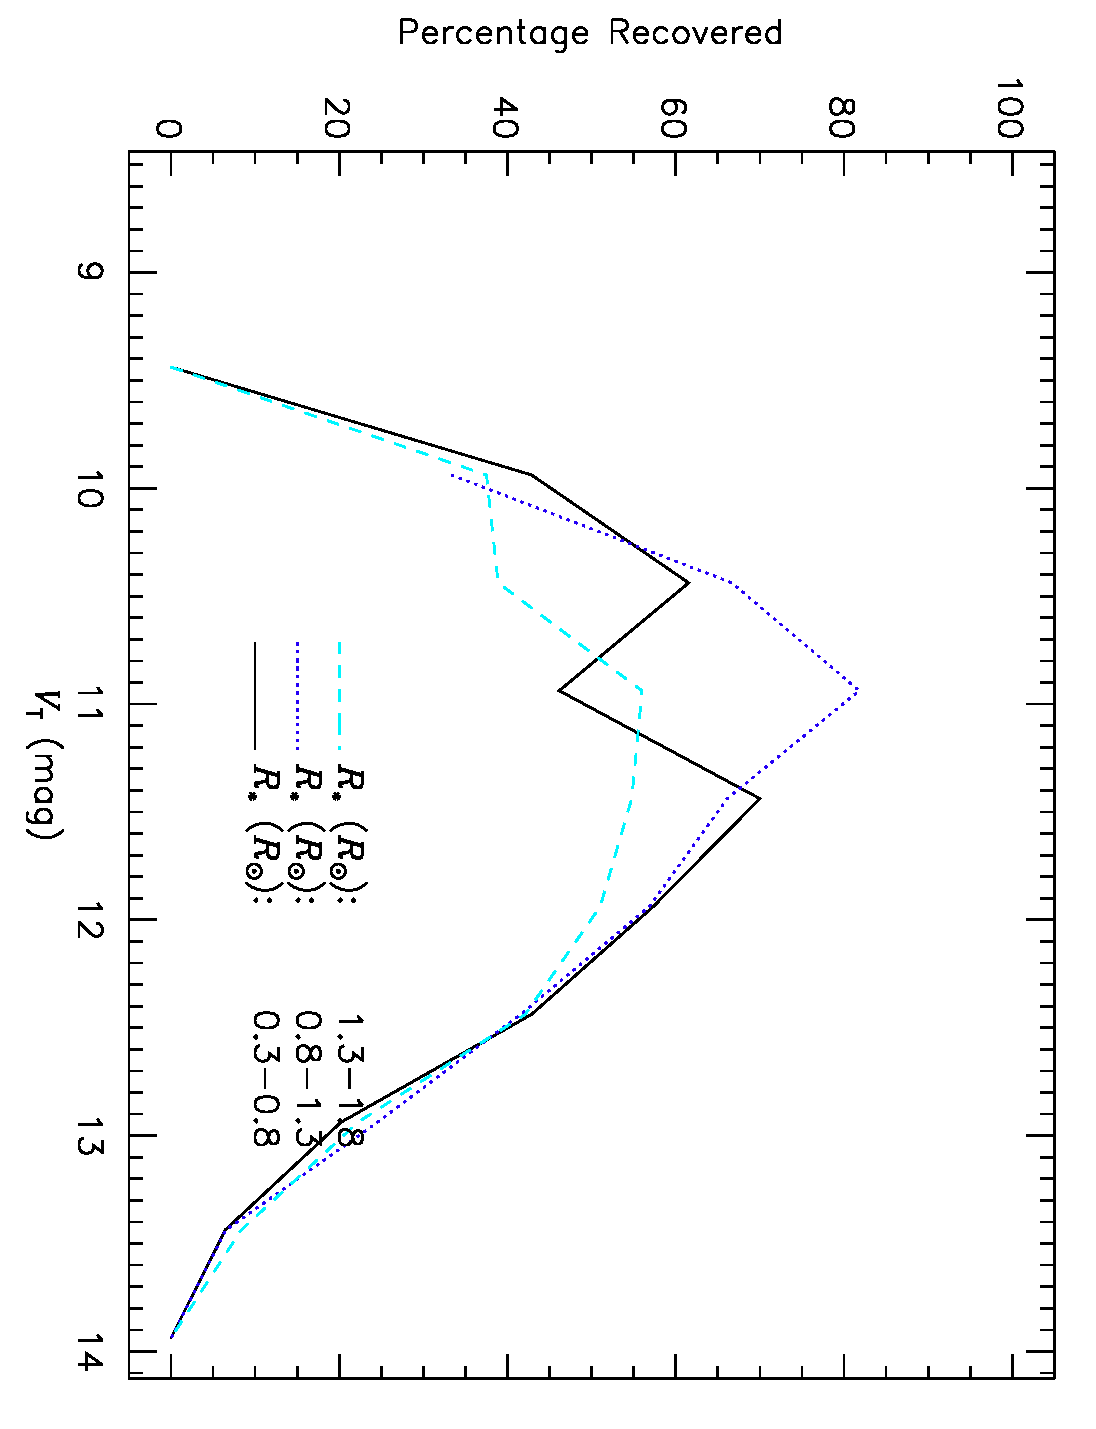
\includegraphics[width=.55\textwidth, angle=90]{7_visual_h}\\
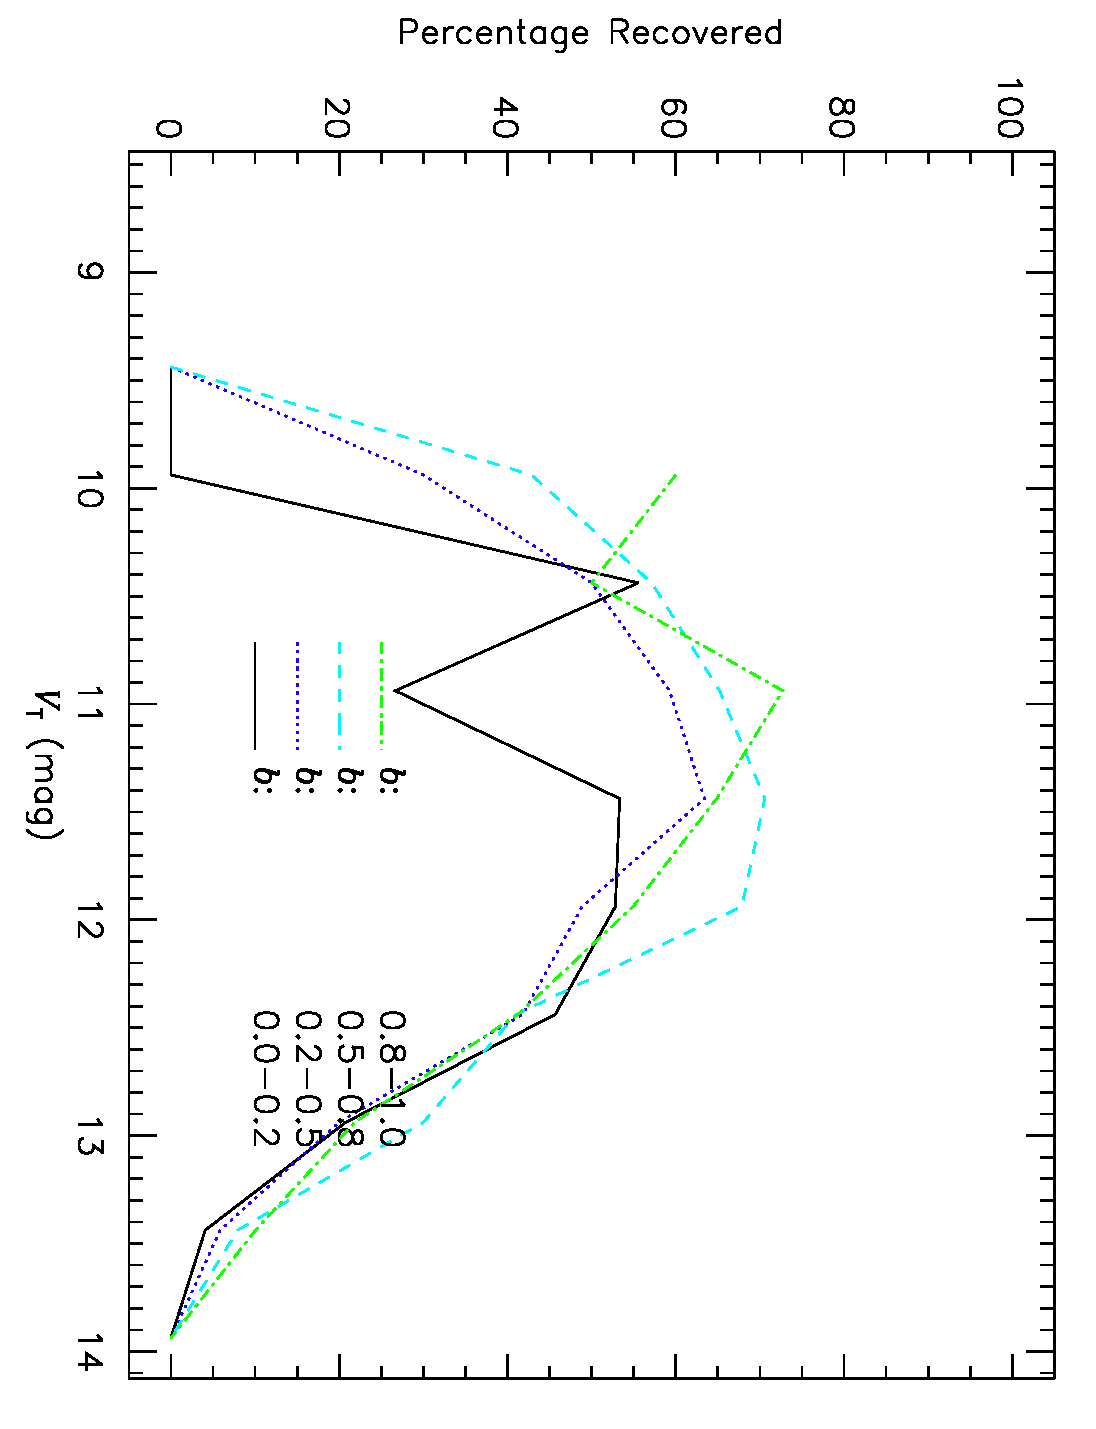
\includegraphics[width=.55\textwidth, angle=90]{7_visual_i}\\
\caption[Visual recovery of different stellar radii and impact parameters]{%
Percentage of the injected transit candidates visually recovered as a function of approximate $V_{T}$ magnitude for different ranges in: %
%($a$)
({\textit top panel}) stellar radii $R_{\star}$, and %
%($b$)
({\textit bottom panel}) impact parameters $b$. %
The recovery rates have been averaged in bins in $V_{T}$ of 0.5\,mag.%
}\label{cha:human:sec:model:fig:visrecrates2}
\end{center}
\end{figure}

The variation of the recovery rate with stellar magnitude for different orbital periods, planetary radii, stellar radii and impact parameters is shown in figures~\ref{cha:human:sec:model:fig:visrecrates1} and~\ref{cha:human:sec:model:fig:visrecrates2}.
These plots show roughly the same trend in magnitudes, periods, impact parameters and object sizes as displayed by the BLS algorithm recovery rates.
However, the maximum recovery rates is reduced by $\sim$20\% in each case.

\section{Discussion}\label{cha:human:sec:discuss}

I have shown that the ability of the BLS transit-search algorithm to recover a candidate transit signal has the expected dependence on the brightness of the target star and the scatter of the photometry.
Few of the candidates with optimal brightness and low scatter were not recovered by the algorithm.
I have also tested my own ability to visually identify a strong transit signal in my data.
I clearly do not identify every candidate correctly recovered by the BLS algorithm, but this is mainly the case for the faintest stars in our field.
However, even for the average-magnitude stars (such as the host star of TrES-2 with $V=11.4$\,mag) I have missed some candidates, and this begs further investigation.
In the end, one must accept the loss of some real detections to avoid being overwhelmed by the data.
I find the recovery rate of my visual analysis to be 87\% for those transit candidates that had a sufficiently high signal-to-noise ratio.

I have found a mild dependence in my transit recovery rates on planetary and stellar radii and on orbital period.
This is in contrast to the similar analysis performed by \citet{Gilliland_Brown_Guhathakurta:apjl:2000a}, who found a strong bias with the planet radius.
